% main.tex: the book. Compile with:  python scripts/build.py   (or: latexmk main.tex, see .latexmkrc)
% Engine: LuaLaTeX + biber. The class lives in latex/aibook.cls.
% Chapter files in latex/chapters/ are GENERATED from chapters/*.txt by scripts/txt2tex.py.
\documentclass{aibook}
\addbibresource{references.bib}
\InputIfFileExists{latex/layout_tight.tex}{}{}   % generated by scripts/layout.py (IR-15)
\bookauthors{ליאת קפהזידר ולבנת בנסון}
\hypersetup{pdftitle={מאחורי הקלעים של הבינה המלאכותית},pdfsubject={ספר מדע פופולרי על בינה מלאכותית},
  pdfkeywords={בינה מלאכותית, למידת מכונה, מודלי שפה, הערכת מודלים}}

\begin{document}

% ------------------------------------------------------------------ front matter
\frontmatter
\makecover{מאחורי הקלעים של הבינה המלאכותית}{מהנתון הראשון ועד לתשובה שעל המסך}{ספר מדע פופולרי · 2026}

\begin{credits}
\textbf{כתיבה ועריכה:} ליאת קפהזידר ולבנת בנסון

\textbf{קוד קבוצה:} \en{LIATLVNT} \quad·\quad \textbf{מטלה:} 02

\textbf{מאגר הקוד:} \en{\url{https://github.com/greenlivnat/HW2}}

\textbf{הפקה:} הספר נכתב, נבדק והודר בתהליך של סוכני בינה מלאכותית (\en{Claude Code}) בהנחיית המחברות ובפיקוחן. תהליך העבודה מתועד בנספח.

\textbf{כלים:} \en{LuaLaTeX}, ‏\en{biber}, ‏\en{Python}, ‏\en{Matplotlib}, ‏\en{scikit-learn}. גופן: \en{Assistant} (רישיון \en{SIL OFL}).

\textbf{נתוני הניסוי בפרק 5:} \en{UCI Optical Recognition of Handwritten Digits (Alpaydin \& Kaynak, 1998)}, רישיון \en{CC BY 4.0}.

\textbf{מספור העמודים} זהה למספור העמודים בקובץ ה-\en{PDF}.
\end{credits}

\chapter*{תקציר}
\addcontentsline{toc}{chapter}{תקציר}
\thispagestyle{frontmatter}
\IfFileExists{latex/frontmatter/abstract.tex}{% Generated by scripts/txt2tex.py from chapters/abstract.txt. Edit the TXT, not this file.
הספר מתחיל משאלה שכל אחד יכול לשאול: מישהו מקליד למערכת שאלה על בצק שלא תופח, ומקבל תשובה בטוחה ומסודרת. מה קרה בין ההקלדה לתשובה? הקוראת עוברת בשבעה פרקים מאחורי המסך, צעד אחר צעד, ובכל פרק נחשף חלק אחר במנגנון: מה זה בכלל מכונה שלומדת, איך נאספים נתונים ומה קורה כשהם מוטים, איך רשת נוירונים מתאימה את עצמה, איך מודל שפה מנבא מילה אחר מילה, ואיך בודקים אם מכונה באמת למדה ולא רק נשמעת כך.

הפרק על הבדיקה כולל ניסוי קטן של הספר עצמו, שבו המספרים מוצגים כפי שיצאו. אחריו באים הגבולות: מה קורה למה שהקוראת הקלידה, מתי מערכת טועה דווקא בטון הבטוח ביותר, ומה כדאי לדעת לפני שסומכים עליה. הפרק האחרון חוזר אל המסך ומציע לא כללים לשינון אלא שיקול דעת: מתי לסמוך, מתי לבדוק, ואיך להשתמש בכלי בלי לוותר על החשיבה של הקוראת עצמה.

נספח נפרד מספר איך נוצר הספר עצמו: בעזרת סוכנים של בינה מלאכותית, שכל אחד מהם עשה תפקיד אחד, תחת פיקוח אנושי ועם תיעוד פתוח לבדיקה. כך הספר מראה בעצמו את מה שהוא מלמד, שאמון נבנה מבדיקה ולא מביטחון.
}{\placeholder{התקציר טרם נכתב (chapters/abstract.txt)}}

\begin{keywordsbox}
\IfFileExists{latex/frontmatter/keywords.tex}{% Generated by scripts/txt2tex.py from chapters/abstract.txt. Edit the TXT, not this file.
בינה מלאכותית (artificial intelligence), למידת מכונה (machine learning), רשתות נוירונים (neural networks), מודלי שפה (language models), הערכת מודלים (model evaluation), הכללה והתאמת יתר (generalization and overfitting), הטיה בנתונים (data bias), אוריינות בינה מלאכותית (AI literacy)
}{\textcolor{red}{חסר}}
\end{keywordsbox}

\tableofcontents
\listoffigures
{\let\clearpage\relax\listoftables}% same page as the list of figures (D-m5b-05)

% ------------------------------------------------------------------ chapters
\mainmatter
% Generated by scripts/txt2tex.py from chapters/chapter_01.txt. Edit the TXT, not this file.
\chapterquestion{מי כתב את התשובה שמופיעה עכשיו על המסך, אם שום אדם לא ראה את השאלה?}
\chapter{מהי בינה מלאכותית?}\label{ch:01}
\section{רגע לפני Enter}
דמיינו שעת ערב מאוחרת. הבצק שהקוראת השאירה על השיש לא תפח, והיא פותחת חלון של מערכת בינה מלאכותית ומקלידה: "למה הבצק שלי לא תופח, ומה אפשר לעשות עכשיו?" כעבור שניות מתחילות להופיע על המסך מילים, אחת אחרי השנייה. לתמונה הזאת נחזור לאורך הספר.
אף מתכנת לא כתב מראש את התשובה הזאת. איש לא ניחש שהקוראת תשאל דווקא על בצק, דווקא הערב, דווקא בניסוח הזה. ובכל זאת התשובה מנוסחת, נוגעת בעניין, ולפעמים אפילו נכונה. מאיפה היא הגיעה?
הספר יוצא למסע אל מאחורי הקלעים של הרגע הקטן הזה.
\section{שם שנולד בהצעת מחקר}
ב-1950 פתח טיורינג מאמר בשאלה "Can machines think?", כלומר: האם מכונות יכולות לחשוב? הוא הציע ניסוי שכינה "משחק החיקוי": חוקר בחדר נפרד שואל שאלות ומנסה לקבוע מי מבין שני משתתפים סמויים הוא הגבר ומי האישה. ואז טיורינג שואל: מה יקרה אם מכונה תתפוס את מקומו של אחד מהם \cite{S-ch01-02}.
השם עצמו נולד כעבור חמש שנים, בהצעת מחקר מ-31 באוגוסט 1955. ארבעה חוקרים, מקארתי, מינסקי, רוצ'סטר ושאנון, הציעו לקיים בקיץ 1956 מחקר של חודשיים בהשתתפות עשרה אנשים, ונתנו לנושא את השם artificial intelligence, כלומר בינה מלאכותית \cite{S-ch01-01}. ההצעה נשענה על השערה נועזת: שכל היבט של למידה, וכל תכונה אחרת של אינטליגנציה, אפשר עקרונית לתאר בדיוק רב כל כך, שמכונה תוכל לדמות אותו. בין שבעת ההיבטים של הבעיה שההצעה מנתה הופיע כבר אז "שיפור עצמי" (Self-Improvement) \cite{S-ch01-01}.
\section{הגדרה שמסרבת להתקבע}
עשרות שנים אחר כך עדיין אין הגדרה מדויקת ומוסכמת, כפי שמודה פאנל המומחים של פרויקט AI100 בסטנפורד (2016) \cite{S-ch01-07}. הפאנל מביא את ההגדרה של נילס נילסון (Nils J. Nilsson): בינה מלאכותית היא פעילות שמטרתה להפוך מכונות לאינטליגנטיות, ואינטליגנציה היא התכונה שמאפשרת לישות לתפקד כראוי, ומתוך ראייה קדימה, בסביבה שלה \cite{S-ch01-07}. הפאנל מתאר גם את "אפקט ה-AI" (AI effect): כשאנשים מתרגלים לטכנולוגיה, היא מפסיקה להיחשב בינה מלאכותית \cite{S-ch01-07}.
הארגון לשיתוף פעולה ולפיתוח כלכלי (OECD) בחר בניסוח מעשי יותר. לפי ההגדרה הרשמית שלו, מערכת בינה מלאכותית היא מערכת מבוססת מכונה שמסיקה מהקלט שהיא מקבלת, לשם מטרות מפורשות או משתמעות, כיצד לייצר פלטים כמו תחזיות, תוכן, המלצות או החלטות, שעשויים להשפיע על סביבות פיזיות או וירטואליות \cite{S-ch01-09}. בעדכון ההגדרה (2023–2024) נוספה המילה "תוכן", כדי להבהיר שגם מערכות של בינה מלאכותית יוצרת (generative AI), כלומר מערכות שמפיקות טקסט ותוצרים חדשים, נכללות בה \cite{S-ch01-10}.
ובערב של הקוראת: הקלט הוא שאלה על בצק, הפלט הוא תוכן על המסך, ובאמצע עומדת המילה החשובה, "מסיקה". ההגדרה לא שואלת אם המכונה חושבת, אלא מה היא עושה עם מה שהיא מקבלת.
\section{מתכון מול טעימה}
תוכנה רגילה דומה למתכון כתוב: מתכנת כותב לכל מצב הוראה מפורשת, אם קרה כך, עשה כך. זה עובד כל עוד אפשר לנסח את הכללים. נסו לכתוב רשימת כללים שמזהה את הספרה 7 בכתב יד: עם קו באמצע או בלי, זקופה או נטויה, מעוגלת או חדה. כל כלל חדש מוליד חריג חדש.
טום מיטשל ניסח את ההבדל בחיבור משנת 2006: מדעי המחשב עסקו בעיקר בשאלה איך לתכנת מחשבים ביד, ואילו למידת מכונה (machine learning) שואלת איך לגרום למחשבים לתכנת את עצמם, מתוך ניסיון ומעט מבנה התחלתי \cite{S-ch01-03}. לדבריו, גם בזיהוי דיבור וגם בראייה ממוחשבת, מערכות מאומנות מדויקות יותר מתוכנות שנכתבו ביד. ונכון ל-2006, יותר מ-85\% מהדואר בכתב יד בארצות הברית מוין אוטומטית, בתוכנה שאומנה בלמידת מכונה \cite{S-ch01-03}.
עצרו רגע מול המספר הזה. על כל מעטפה כזאת כתב מישהו בכתב ידו, עם הנטייה והעיגולים שרק לו יש. איש לא מנה בפני המכונה את כל הדרכים לכתוב כל אות וכל ספרה, ובכל זאת היא למדה לפענח אותן מתוך דוגמאות. מיומנות שקשה להסביר במילים נלמדה בלי הסבר.
אם תוכנה רגילה היא מתכון, מערכת לומדת דומה לטבח שמעולם לא קרא מתכון, אבל טעם אינספור תבשילים ושמע בכל פעם מה הצליח ומה לא. הכללים שלו לא נכתבו בשום מקום. הם התגבשו.
טיורינג חשב בכיוון דומה. הוא הציע לבנות מכונה שמדמה מוח של ילד ולא של מבוגר, ותיאר את מוח הילד כמחברת חדשה מחנות כלי כתיבה: מעט מנגנון והרבה דפים ריקים \cite{S-ch01-02}.
\section{מה הופך מערכת ל"לומדת"}
\begin{conceptbox}{למידה לפי משימה, מדד וניסיון}
מיטשל מציע הגדרה בת שלושה רכיבים: מכונה לומדת ביחס למשימה T (task), מדד ביצוע P (performance) וסוג ניסיון E (experience), אם היא משפרת באופן אמין את הביצועים שלה במדד P במשימה T בעקבות הניסיון E \cite{S-ch01-03}.
לדוגמה, מסנן דואר זבל:
המשימה (T): להבחין בין הודעה רצויה להודעת זבל.
המדד (P): החלק של ההודעות שסווגו נכון.
הניסיון (E): הודעות קודמות שמשתמשים כבר סימנו כ"זבל" או כ"תקין".
אם המסנן טועה פחות ככל שהוא רואה יותר הודעות מסומנות, הוא לומד.
\end{conceptbox}
ההגדרה לא דורשת הבנה או תודעה, רק שיפור שאפשר למדוד. מיטשל אף רואה בלמידת מכונה צאצא טבעי של המפגש בין מדעי המחשב לסטטיסטיקה \cite{S-ch01-03}: כדי לדעת אם משהו השתפר, צריך לספור ולהשוות.
\section{שלוש בובות, אחת בתוך השנייה}
כדי לסדר את שלושת המושגים, הספר הזה מציע תמונה משלו: בובת מטריושקה. הבובה החיצונית היא בינה מלאכותית: מערכות שמקבלות קלט ומסיקות ממנו פלט. בתוכה יושבת למידת מכונה: מערכות שההתנהגות שלהן נבנית מתוך ניסיון ולא נכתבת כולה ביד. ובפנים, הקטנה ביותר: למידה עמוקה (deep learning). לא כל בינה מלאכותית לומדת, ולא כל למידה היא עמוקה.
מומחי AI100 מונים כמה גורמים שהזינו את מהפכת הבינה המלאכותית, ובראשם הבשלתה של למידת המכונה \cite{S-ch01-08}. את הלמידה העמוקה הם מתארים כסוג של רשתות נוירונים מלאכותיות (artificial neural networks), שמאומנות בשיטה שנקראת התפשטות לאחור (backpropagation) \cite{S-ch01-08}. רשת נוירונים היא מבנה חישובי של יחידות פשוטות רבות שמחוברות זו לזו.
ומה פירוש "עמוקה"? לפי סקירה שפרסמו לקון, בנג'יו והינטון ב-Nature ב-2015, מערכת כזאת בנויה משכבות עיבוד רבות, וכל שכבה בונה את התיאור שלה לנתונים מתוך התיאור של השכבה שלפניה. כך נוצרות כמה רמות של הפשטה \cite{S-ch01-05}. לתיאור כזה קוראים ייצוג (representation). זה דומה לילד שלומד לקרוא: קודם קווים, אחר כך אותיות, מילים ולבסוף משפט שלם.
ומה קובע את התיאור שכל שכבה מפיקה? אוסף גדול של מספרים פנימיים, הפרמטרים, שאפשר לדמות לכפתורים במערבל קול; בפרק 3 נפתח רשת כזאת ונפגוש אותם בשמות משקולות והטיות. התפשטות לאחור היא האלגוריתם שמסמן למכונה איך לשנות את הכפתורים האלה בכל שכבה \cite{S-ch01-05}. דמיינו טכנאי שמשווה את מה שנשמע למה שהיה אמור להישמע, ומזיז כל כפתור מעט בכיוון שמקטין את הפער. לפי הסקירה, השיטות האלה שיפרו מאוד את התוצאות הטובות ביותר שהושגו עד אז בזיהוי דיבור, בזיהוי עצמים בתמונות ובתחומים רבים אחרים \cite{S-ch01-05}.
\begin{figure}[htbp]
\centering
% Figure 1.1: three nested circles (AI > ML > DL). Book framework, no external data.
% Gold is used only for marker dots; label text stays Midnight Blue (contrast, R-ch01-16).
\begin{bookdiagram}
  \fill[midnight!7,draw=midnight,line width=1.2pt] (0,0) circle (3.3);
  \fill[turquoise!14,draw=turquoise,line width=1.2pt] (0,-0.95) circle (2.3);
  \fill[violet!16,draw=violet,line width=1.2pt] (0,-1.95) circle (1.3);
  \node[font=\headingfont\normalsize] at (0,2.55) {בינה מלאכותית};
  \node[font=\headingfont\normalsize] at (0,0.75) {למידת מכונה};
  \node[font=\headingfont\normalsize,align=center] at (0,-1.95) {למידה\\עמוקה};
  \draw[midnight,line width=0.6pt] (-1.75,2.55) -- (-4.3,2.3);
  \draw[turquoise,line width=0.6pt] (-1.45,0.75) -- (-4.3,0.5);
  \draw[violet,line width=0.6pt] (-0.75,-1.95) -- (-4.3,-1.5);
  \foreach \y in {2.3,0.5,-1.5}{\fill[gold] (-4.3,\y) circle (1.6pt);}
  \node[anchor=east,text width=4.1cm,align=right,font=\footnotesize] at (-4.45,2.3) {מסיקה מתוך הקלט שהיא מקבלת איך לייצר פלט};
  \node[anchor=east,text width=4.1cm,align=right,font=\footnotesize] at (-4.45,0.5) {ההתנהגות שלה נבנית מתוך ניסיון};
  \node[anchor=east,text width=4.1cm,align=right,font=\footnotesize] at (-4.45,-1.5) {ייצוגים שנלמדים בשכבות רבות};
\end{bookdiagram}

\caption{שלוש בובות, אחת בתוך השנייה}\label{fig:1.1}
\figurenote{מקור: מסגרת הספר (לא מקור חיצוני)}
\end{figure}
\begin{thinkbox}
הפאנל של סטנפורד מזכיר שמחשבון אלקטרוני פשוט מחשב מהר בהרבה ממוח אדם, ורואה באינטליגנציה רצף: ההבדל בין מחשבון למוח הוא בקנה מידה, במהירות, באוטונומיה ובכלליות, ולא בסוג \cite{S-ch01-07}.
האם המחשבון בטלפון שלכם הוא בינה מלאכותית? ומה לגבי ההשלמה האוטומטית במקלדת? היכן הייתם מותחים את הקו, והאם הוא יישאר שם בעוד עשור?
\end{thinkbox}
\section{מפת הדרך: מה מחכה מאחורי המסך}
השאלה על הבצק נשלחה. אלה התחנות שבדרך: פרק 2, "מנתונים ללמידה": הדוגמאות שמהן המערכת למדה, אימון, בדיקה והטיות. פרק 3, "הרשת הנוירונית מבפנים": איך מספרים ומשקולות מצטרפים לתחזית. פרק 4, "כיצד מודל שפה מייצר תשובה": איך התשובה נבנית חלק אחר חלק. פרק 5, "בודקים מודלים בעזרת נתונים": איך מבחינים בין הצלחה לאשליה שלה. פרק 6, "מה AI יודע — ומה לא": טעויות בטוחות בעצמן, פרטיות וזכויות. פרק 7, "האדם במעגל והעתיד": תפקידה של הקוראת מול התשובה. נספח, "כך נוצר הספר שאתם קוראים": מאחורי הקלעים של הספר עצמו.
אבל המסע מתחיל הרבה לפני שהקוראת הקלידה: בדוגמאות שמהן המערכת למדה.
\begin{insightsbox}
\begin{itemize}
\item "בינה מלאכותית" היא משפחה של הגדרות; המעשיות שבהן שואלות מה המערכת עושה עם הקלט, ולא אם היא "חושבת" \cite{S-ch01-07,S-ch01-09}.
\item בתוכנה רגילה אדם מנסח את הכללים; במערכת לומדת המחשב "מתכנת את עצמו" מתוך ניסיון ומעט מבנה התחלתי \cite{S-ch01-03}.
\item לפי ההגדרה של מיטשל, מערכת למדה אם הביצועים שלה במשימה, לפי מדד מוגדר, משתפרים באופן אמין בעקבות ניסיון \cite{S-ch01-03}.
\item למידה עמוקה לומדת שכבה על גבי שכבה של ייצוגים \cite{S-ch01-05}. במטריושקה של הספר היא רק הבובה הפנימית, ולא שם נרדף לבינה מלאכותית.
\item הקו בין "כלי" ל"בינה" זז עם ההרגל: מה שמפליא היום ייראה מחר כמו עוד פונקציה בטלפון \cite{S-ch01-07}.
\end{itemize}
\end{insightsbox}

% Generated by scripts/txt2tex.py from chapters/chapter_02.txt. Edit the TXT, not this file.
\chapterlayout{02}
\chapterquestion{איך הופכות אלפי דוגמאות לידע, ומה קורה כשהן מטעות?}
\chapter{מנתונים ללמידה}\label{ch:02}
\section{להריץ את הסרט אחורה}
השאלה על הבצק עדיין מהבהבת על המסך. אבל כדי להבין מאיפה תגיע התשובה, צריך להריץ את הסרט אחורה, הרבה לפני הערב הזה. עוד לפני שמישהו ידע שהקוראת תשאל, המערכת כבר עברה מסע ארוך של התנסות בדוגמאות.
גם הקוראת לא נולדה אופה. כשהיא נזכרת איך למדה, היא לא רואה מול עיניה ספר הוראות, אלא שורה ארוכה של ניסיונות: כיכר שיצאה שטוחה, עוגה שהתפוררה, ופעם אחת, סוף סוף, לחם שכולם ביקשו ממנו עוד. אף ניסיון לא לימד אותה כלל מפורש. ביחד הם בנו אצלה תחושה. ומה שהיא לא שמה לב אליו אז: גם הניסיונות עצמם נבחרו בשבילה. היא אפתה רק במטבח שלה, בתנור שלה, בקמח מהמכולת הקרובה.
מערכת לומדת עוברת מסלול דומה, אבל כל צעד בו הוא החלטה של בני אדם. את המערכת הגדולה שהקוראת משוחחת איתה קשה לפתוח, ולכן נלווה בפרק הזה מערכת קטנה ודמיונית לגמרי: צוות שבונה מסווג (classifier), תוכנה שמשייכת כל קלט לאחת מכמה קטגוריות. המסווג מקבל תמונה של בצק ומכריע: "תפח" או "לא תפח". הצוות והתמונות הם המחשה בלבד.
\section{מאיפה באות הדוגמאות}
הצוות מתחיל באיסוף. אלפי תמונות מצטברות: חלקן צולמו בידי חברי הצוות, חלקן נשלחו מחברים. כבר בשלב הזה נקבע הרבה. לפי מאמר "Datasheets for Datasets", מאפייני מאגר הנתונים משפיעים באופן יסודי על התנהגות המודל, ומודל לא צפוי לתפקד היטב בשטח אם הסביבה שבה הוא פועל אינה תואמת את הנתונים שעליהם אומן ונבדק \cite{S-ch02-04}.
ובכל זאת, כשטימניט גברו ועמיתיה כתבו את המאמר ב-2018, לא היה בקהילת למידת המכונה תהליך סטנדרטי לתיעוד מאגרי נתונים. הם הציעו לצרף לכל מאגר "דף נתונים" (datasheet), בהשראת הדפים שמלווים כל רכיב אלקטרוני \cite{S-ch02-03}. השאלות שבדף נשמעות פשוטות, ודווקא משום כך הן חושפות: מי אסף את הנתונים ובאיזה מנגנון, כמה שולם לו, באיזו שיטה נבחרו הדוגמאות, האם המאגר הוא מדגם, והאם הוא מייצג \cite{S-ch02-04}.
\section{ניקוי: לסלק את מה שמטעה}
אחרי האיסוף מגיע שלב פחות זוהר. ניקוי נתונים, במילים פשוטות, הוא חיפוש אחר מה שעלול להטעות את המכונה, והחלטה מה לעשות בו. קורס המבוא של גוגל ללמידת מכונה מונה כמה חשודים קבועים: ערכים חסרים, דוגמאות כפולות, ערכים שגויים ותוויות שגויות \cite{S-ch02-13}. אצל הצוות זה נראה כך: תמונה שהועלתה פעמיים, תמונה בלי פרטים על מקורה, ועוגה שהתגנבה לתיקייה של לחמים.
אותו מקור מזכיר שאי אפשר לנקות מאגר מכל הרעש \cite{S-ch02-13}. המטרה היא נתונים שאפשר לסמוך עליהם, לא נתונים מושלמים. וכיוון שכל הסרה וכל תיקון משנים את מה שהמודל יראה, דף הנתונים שואל גם אילו פעולות עיבוד בוצעו, והאם הנתונים הגולמיים נשמרו בצד \cite{S-ch02-04}.
\section{תוויות: מי מחליט מה נכון?}
למסווג כזה, תמונה לבדה אינה מלמדת דבר. לכל תמונה צריך להצמיד תווית (label), כלומר את התשובה שהמודל אמור לחזות. וכאן מתברר שהמילה "נכונה" חמקמקה. שני מתייגים מביטים באותו בצק: האחד כותב "תפח", והשנייה מהססת.
אותו קורס, בשיעור על תוויות, ממליץ לא לסמוך בעיניים עצומות על מתייגים אנושיים: הם טועים, לפעמים צריך כמה מהם, וכדאי לתייג בעצמכם כאלף דוגמאות ולהשוות \cite{S-ch02-12}. וכשהמתייגים חלוקים, אין להניח שהתיוג שלכם הוא הנכון, במיוחד בשיפוטים ערכיים \cite{S-ch02-12}.
מלכודת נוספת היא תווית עקיפה (proxy label): במקום למדוד את מה שרוצים, מודדים משהו קרוב. לדוגמה, הצוות עלול להחליט ש"תפח" פירושו "האופה נתן לתוצאה חמישה כוכבים". אבל דירוג מעיד על שביעות רצון, לא בהכרח על תפיחה. תווית עקיפה היא תמיד פשרה, והמודל מועיל רק במידה שהקשר בינה לבין מה שרוצים לחזות חזק \cite{S-ch02-12}.
\begin{behindbox}{שלוש ערימות, אחת נעולה}
אחרי הניקוי והתיוג, הצוות מחלק את התמונות לשלוש ערימות \cite{S-ch02-10}:
קבוצת אימון (training set): ממנה המודל לומד.
קבוצת אימות (validation set): עליה משווים גרסאות ומכווננים היפר-פרמטרים, הגדרות שהאדם קובע ולא המודל.
קבוצת בדיקה (test set): נעולה במגירה, ונפתחת רק לבדיקה הסופית \cite{S-ch02-09}.
קורס המבוא מציג, כדוגמה ולא ככלל, חלוקה של 70\% לאימון ו-15\% לכל אחת מהאחרות \cite{S-ch02-10}. למה לא להסתפק בשתיים? כי כיוונון לפי קבוצת הבדיקה מזרים אל המודל ידע עליה \cite{S-ch02-09}. המחיר: פחות דוגמאות ללמידה, ותוצאה שתלויה במזל של החלוקה. אחת התשובות היא אימות צולב (k-fold): מחלקים את קבוצת האימון ל-k חלקים, בכל סבב לומדים מכולם חוץ מאחד, בוחנים על הנותר, ומדווחים על הממוצע \cite{S-ch02-09}.
\end{behindbox}
\section{הכללה: המבחן שלא ראו לפניו}
למה כל הטקס הזה? כי מודל שנבחן על אותן תמונות שעליהן התאמן יכול להיראות מבריק ולהיות חסר תועלת. התיעוד של הספרייה scikit-learn מתאר זאת בחדות: מודל שפשוט חוזר על התוויות שראה יקבל ציון מושלם, ולא יחזה שום דבר שימושי על נתונים חדשים \cite{S-ch02-09}. לזה קוראים התאמת-יתר (overfitting): שינון של קבוצת האימון, צמוד כל כך שהמודל נכשל מול דוגמאות חדשות \cite{S-ch02-11}. ההפך הוא הכללה (generalization): היכולת לחזות היטב גם על מה שלא נראה מעולם \cite{S-ch02-11}.
הכללה אינה מובטחת. יש תנאים שבהם אפשר לצפות לה: הדוגמאות בלתי תלויות זו בזו ומגיעות מאותה התפלגות, הנתונים אינם משתנים משמעותית לאורך זמן, ושלוש הערימות דומות זו לזו סטטיסטית \cite{S-ch02-11}. ויש גם שחיקה: ככל שבודקים יותר פעמים מול אותה קבוצת בדיקה, המודל מתאים את עצמו אליה, והיא מאבדת מערכה כמבחן \cite{S-ch02-10}. איך מודדים הצלחה בפועל? לשם נגיע בפרק 5.
\begin{figure}[htbp]
\centering
% Figure 2.1: the path of the examples, from collection to the final test (conceptual, no data).
\begin{bookdiagram}[x=1cm,y=1cm]
  \tikzset{st/.style={blk,draw=turquoise,text width=2.75cm,minimum height=11mm}}
  \node[st] (raw)   at (13.6,0)  {דוגמאות גולמיות};
  \node[st] (clean) at (9.6,0)   {ניקוי};
  \node[st] (lab)   at (5.6,0)   {תיוג};
  \node[st] (split) at (1.6,0)   {חלוקה לאימון, אימות ובדיקה};
  \node[st] (train) at (1.6,-2.2) {אימון};
  \node[st] (tune)  at (5.6,-2.2) {כיוונון מול קבוצת האימות};
  \node[st,draw=midnight,line width=1.2pt] (final) at (11.2,-2.2) {בדיקה סופית, חד-פעמית};
  \node[blk,fill=midnight,text=white,text width=3.4cm,minimum height=11mm] (test) at (11.2,-5.0) {קבוצת הבדיקה};
  \draw[flow] (raw) -- (clean);
  \draw[flow] (clean) -- (lab);
  \draw[flow] (lab) -- (split);
  \draw[flow] (split) -- (train);
  \draw[flow] (train) -- (tune);
  \draw[flow] (tune) -- (final);
  \draw[flow] (split.west) -- ++(-0.45,0) |- node[pos=0.75,below,font=\footnotesize] {מופרדת מראש} (test.west);
  % the wall, with the lock where the single legitimate arrow passes
  \draw[midnight,line width=3pt] (8.6,-3.65) -- (14.2,-3.65);
  \draw[midnight,line width=3pt] (8.6,-3.65) -- (8.6,-6.0);
  \draw[flow,draw=midnight] (test.north) -- node[right=4mm,font=\footnotesize] {פעם אחת, בסוף} (final.south);
  \node[fill=gold,draw=midnight,rounded corners=0.6mm,minimum width=5mm,minimum height=4mm,inner sep=0pt] (lock) at (11.2,-3.65) {};
  \draw[midnight,line width=1pt] ([xshift=-1.4mm]lock.north) arc (180:0:1.4mm);
  \draw[loop,line width=1.2pt] (test.west) to[out=180,in=-90] node[pos=0.55,below left,font=\footnotesize\headingfont,text=violet] {זליגה: הדרך האסורה} (tune.south);
  \node[text=violet,font=\headingfont\Large] at (8.6,-4.55) {\(\times\)};
\end{bookdiagram}

\caption{מסלול הדוגמאות, מהאיסוף ועד הבדיקה}\label{fig:2.1}
\figurenote{מקור: מסגרת הספר, על בסיס \cite{S-ch02-08}, \cite{S-ch02-09} ו-\cite{S-ch02-10} (תרשים מושגי, בלי נתונים)}
\end{figure}
\section{זליגה: כשהשאלות דולפות לפני הבחינה}
דמיינו מבחן בגרות שהשאלות שלו דלפו יום קודם. הציונים יזנקו, אבל הם כבר לא אומרים דבר על הידע של התלמידים. בלמידת מכונה קוראים לזה זליגת נתונים (data leakage): שימוש, בזמן בניית המודל, במידע שלא יהיה זמין ברגע החיזוי. התוצאה היא הערכה אופטימית מדי, וביצועים חלשים יותר על נתונים חדשים באמת \cite{S-ch02-08}. שחר קאופמן, סהרון רוסט ועמיתיהם מזכירים שהזליגה נחשבת לאחת מעשר הטעויות המובילות בכריית נתונים, ומציעים למנוע אותה בהפרדה קפדנית בין הנתונים שמהם לומדים לבין אלה שעליהם חוזים \cite{S-ch02-06}.
אצל הצוות הדמיוני, הדליפה מגיעה מהדלת האחורית: עותק כפול אחד חמק מהניקוי ונחת פעם בערימת האימון ופעם בערימת הבדיקה. הקורס של גוגל מזהיר בדיוק מזה: בקבוצת בדיקה טובה אין אף דוגמה משוכפלת מקבוצת האימון, כי המבחן ההוגן היחיד הוא מול דוגמאות חדשות ולא מול העתקים \cite{S-ch02-10}.
הזליגה יכולה להיות עדינה עוד יותר. התיעוד של scikit-learn מציג הדגמה סינתטית, לא מקרה מהעולם: 200 דוגמאות, 10,000 מאפיינים אקראיים ותוויות אקראיות. אין שם שום דבר ללמוד, והדיוק הצפוי הוא של ניחוש, כ-0.5. כשבחרו את המאפיינים "המבטיחים" מתוך כל הנתונים לפני החלוקה, דווח דיוק של 0.76. כשחילקו קודם ובחרו אחר כך, הדיוק חזר ל-0.5 \cite{S-ch02-08}. המודל "גילה" דפוס שלא היה קיים מעולם. הכלל שהתיעוד מנסח: לחלק לאימון ולבדיקה לפני כל עיבוד מקדים, ולעולם לא להתאים (fit) דבר על נתוני הבדיקה \cite{S-ch02-08}.
\section{הטיה: מחברת שנכתבה במטבח אחד}
נחזור למטבח של הקוראת. נניח שכל מה שהיא יודעת על אפייה רשום במחברת אחת, שנכתבה במטבח אחד, מול תנור אחד. בבית שלה המחברת מצוינת; אצל השכנה היא עלולה להטעות. כך גם הצוות: אם כמעט כל התמונות צולמו בשני מטבחים מוארים היטב, המסווג עלול למעוד מול תמונה שצולמה באור עמום של ערב.
לתופעה הזאת קוראים הטיה (bias) בנתונים, ואין לבלבל אותה עם ההטיה שנפגוש בפרק 3, שהיא מספר בתוך הרשת. השיעור על הוגנות באותו קורס מבחין בכמה סוגים, ובהם הטיית בחירה (selection bias), כשהדוגמאות לא נבחרו כך שישקפו את ההתפלגות האמיתית, והטיה היסטורית (historical bias), כשנתוני העבר נושאים אי-שוויון שהיה קיים \cite{S-ch02-14}. מודלים עלולים לשחזר הטיות כאלה ואף להגביר אותן \cite{S-ch02-04}.
המקרה המתועד הבולט, מחקר שנקרא Gender Shades, מגיע מ-2018. ג'וי בואולמוויני וטימניט גברו בחנו שלושה מסווגי מגדר מסחריים, של Microsoft, IBM ו-Face++. קודם הראו ששני מאגרי בנצ'מרק (benchmark, מאגר מבחן מקובל להשוואה) מוכרים, IJB-A ו-Adience, מורכבים ברובם מבהירי עור: 79.6\% ו-86.2\% בהתאמה \cite{S-ch02-01}. לכן בנו מאגר בדיקה משלהן, PPB: 1,270 חברי פרלמנט משלוש מדינות באפריקה ומשלוש באירופה. גוון העור תויג בסולם בן שש דרגות, ורופאת עור מוסמכת קבעה את התוויות הסופיות. המחברות עצמן מציינות שתיוג בינארי של מגדר הוא צמצום שאינו לוכד את המורכבות \cite{S-ch02-01}.
התוצאות על מאגר PPB: אצל נשים כהות עור שיעור השגיאה נע בין 20.8\% ל-34.7\%, לפי המסווג, ואצל גברים בהירי עור בין 0.0\% ל-0.8\% בלבד. נשים כהות עור היו 21.3\% מהמאגר, אבל 61.0\% עד 72.4\% מהשגיאות \cite{S-ch02-01}. הלקח שהספר גוזר מכך: ציון כולל נאה יכול להסתיר כשל עמוק אצל קבוצה אחת, שמתגלה רק כשבודקים כל קבוצה בנפרד.
ומה גרם לפער? כאן נדרשת זהירות. החברות לא פרסמו על אילו נתונים אומנו המסווגים, והמחברות מעלות השערה ולא קביעה: ייתכן שעור כהה מתואם עם מאפייני פנים או עם נורמות של הצגת מגדר שהיו מיוצגים פחות בנתוני האימון \cite{S-ch02-01}.
\begin{mythbox}
\mythlabel אם רק נאסוף מספיק נתונים, ההטיה תתמוסס מעצמה.
\tcblower
\realitylabel הטיית בחירה נובעת מהאופן שבו נבחרו הדוגמאות, לא ממספרן \cite{S-ch02-14}. אם הצוות יכפיל פי עשרה את התמונות משני אותם מטבחים, הוא יקבל מחברת עבה יותר, שנכתבה באותו מטבח. ב-Gender Shades, מה שחשף את הפער היה הרכב ולא גודל: מאגר הבדיקה PPB מאוזן כמעט לגמרי, 53.6\% בהירי עור ו-46.4\% כהי עור \cite{S-ch02-01}. הוא לא תיקן אף מסווג, אבל בעזרתו אפשר היה לראות היכן הם נכשלים. כמות עונה על השאלה "כמה דוגמאות יש?", והטיה שואלת "מי מיוצג, ואיך?". לכן בקבוצת בדיקה טובה גודל לבדו אינו מספיק: היא צריכה גם לייצג את העולם שבו המודל יפעל \cite{S-ch02-10}.
\end{mythbox}
\section{בחזרה לערב ההוא}
הסרט רץ קדימה. הקוראת עדיין מול המסך, והמילים הראשונות של התשובה רק מתחילות להופיע. עכשיו אנחנו יודעים שמאחוריה עומדות החלטות של אנשים שהיא לעולם לא תפגוש: מה לאסוף, מה להשליך, איך לתייג, ומה לנעול במגירה עד הרגע האחרון.
\begin{thinkbox}
דמיינו שלמערכת שהקוראת משוחחת איתה היה מצורף דף נתונים. איזו שאלה הייתם רוצים לקרוא בו ראשונה: מי אסף את הדוגמאות שמהן למדה, מה הוסר מהן בניקוי, או מי החליט מהי תשובה "טובה"? ואם התשובה לשאלה שחשובה לכם ביותר הייתה "לא ידוע", האם הייתם סומכים על העצה באותה מידה?
\end{thinkbox}
נשארת עוד תעלומה. דוגמאות הן תמונות, מילים ומשפטים, אבל המכונה אינה רואה אף אחד מהם. בפרק הבא נרד שכבה נוספת אל מתחת למסך, ונגלה איך הדוגמאות הופכות למספרים, ואיך המספרים מתחילים להכריע.
\begin{insightsbox}
\begin{itemize}
\item כל מערכת לומדת נשענת על שרשרת של החלטות אנושיות: מה נאסף, מה נוקה, ואיך תויג. דף נתונים הוא דרך לחשוף את השרשרת הזאת \cite{S-ch02-03,S-ch02-04}.
\item תווית היא שיפוט, לא עובדה טבעית. מתייגים טועים וחלוקים, ותווית עקיפה מודדת רק משהו קרוב למה שרוצים \cite{S-ch02-12}.
\item קבוצת הבדיקה נשמרת נעולה עד הסוף, כי רק דוגמאות שהמודל לא פגש מעידות על הכללה ולא על שינון \cite{S-ch02-09,S-ch02-11}.
\item זליגה מייצרת הצלחה מדומה: אפילו על נתונים אקראיים לגמרי, עיבוד לפני החלוקה העלה את הדיוק המדווח מרמת ניחוש ל-0.76 \cite{S-ch02-08}.
\item הטיה נובעת מהאופן שבו הנתונים נבחרו וממה שהם משקפים, למשל קבוצה שמיוצגת פחות או אי-שוויון מהעבר, ולא מכמותם; ב-Gender Shades הפער נחשף רק בבדיקה נפרדת של כל תת-קבוצה \cite{S-ch02-01,S-ch02-14}.
\end{itemize}
\end{insightsbox}

% Generated by scripts/txt2tex.py from chapters/chapter_03.txt. Edit the TXT, not this file.
\chapterquestion{מה נשאר מהשאלה על הבצק ברגע שהיא נכנסת אל תוך המכונה?}
\chapter{הרשת הנוירונית מבפנים}\label{ch:03}
\section{אין בצק בפנים}
השאלה של הקוראת כבר יצאה לדרכה. היא הקלידה "בצק", "תופח", "עכשיו", אבל ברגע שהמילים חוצות את גבול המסך הן מפסיקות להיות מילים. בתוך המערכת אין קמח, אין שיש ואין ערב מאוחר. יש מספרים. איך בדיוק טקסט הופך לרצף של מספרים נראה בפרק הבא; כאן נניח שההמרה כבר קרתה, ונרד אל היחידה הקטנה ביותר שמעבדת אותם: הנוירון המלאכותי (artificial neuron).
בפרק 1 דימינו את הפרמטרים של רשת לכפתורים במערבל קול. עכשיו נפרק את הלוח ונבדוק מה מחובר לכל כפתור.
\section{שקילה לפני החלטה}
דמיינו שאתם מתלבטים אם לצאת לטיול ערב. כמה שיקולים עולים בבת אחת: תחזית הגשם, העייפות, חבר שהציע להצטרף. לכל שיקול כובד משלו. תחזית סוערת דוחפת בתוקף נגד, ההזמנה מושכת בעדינות בעד. ויש גם נטייה כללית שקיימת עוד לפני כל שיקול: יש מי שיוצאים כמעט תמיד, ויש מי שנשארים בבית כמעט תמיד.
נוירון מלאכותי עושה משהו דומה, רק בלי לדעת על מה הוא מחליט. לפי רשימות הקורס CS231n של אוניברסיטת סטנפורד, כל נוירון מכפיל כל קלט במשקולת שלו, מחבר את המכפלות, מוסיף הטיה (bias) ומפעיל על התוצאה פונקציה לא-ליניארית \cite{S-ch03-01}. המשקולות (weights) הן עוצמות ההשפעה: הן קובעות כמה כל קלט "נחשב", ומה שחשוב יותר, הן נלמדות \cite{S-ch03-01}. משקולת חיובית גדולה מגבירה קלט, משקולת שלילית הופכת אותו לשיקול נגד, ומשקולת קרובה לאפס כמעט מתעלמת ממנו. ההטיה היא הנטייה הכללית: מספר קבוע שמזיז את התוצאה למעלה או למטה, בלי קשר למה שנכנס. אל תבלבלו אותה עם ההטיה מפרק 2, זו שמסתתרת בנתונים ופוגעת בהוגנות. כאן מדובר במספר אחד נוסף בחשבון, שבמקרה חולק איתה את השם, גם באנגלית.
זה מה שמסתתר מאחורי הלוח: כל משקולת וכל הטיה הן מספר אחד שאפשר לכוונן, והתפשטות לאחור היא האלגוריתם שמסמן לאיזה כיוון לשנות כל אחד מהם בזמן האימון \cite{S-ch01-05}.
\section{הנוסחה, סימן אחר סימן}
את מה שתואר במילים אפשר לכתוב בשורה אחת:
\begin{equation}
z = \sum_{i=1}^{n} w_i x_i + b
\end{equation}
x\_i: הקלט שמספרו i, אחד המספרים שנכנסים לנוירון. w\_i: המשקולת של אותו קלט. w\_i x\_i: המכפלה, כלומר כמה הקלט שוקל אחרי שהוכפל בחשיבות שלו. \textbackslash{}sum\_\{i=1\}\textasciicircum{}\{n\}: האות היוונית סיגמה מורה "חברו את כולם", מהקלט הראשון (i = 1) ועד האחרון. n: מספר הקלטים. b: ההטיה, שמתווספת לסכום פעם אחת. z: התוצאה, הסכום המשוקלל. מספר בודד.
ואז הצעד השני:
\begin{equation}
a = f(z)
\end{equation}
האות f מסמנת את פונקציית ההפעלה, ו-a הוא הפלט של הנוירון, המספר שימשיך הלאה. בחומרי הקורס של סטנפורד שני הצעדים כתובים כביטוי אחד, שבו הפונקציה עוטפת את הסכום \cite{S-ch03-01}. הספר מפריד ביניהם כדי שנוכל לעצור ולהתבונן בכל צעד לחוד.
\begin{labbox}{נוירון צעצוע בערב של הקוראת}
מספרים להמחשה בלבד. דמיינו נוירון עם שלושה קלטים שהגיעו מתוך השאלה על הבצק: $x_{1}$ = 0.9, $x_{2}$ = 0.2, $x_{3}$ = 0.5. המשקולות: $w_{1}$ = 1.5, $w_{2}$ = -2.0, $w_{3}$ = 0.8, וההטיה b = -0.5.
z = 1.5$\times$0.9 + (-2.0)$\times$0.2 + 0.8$\times$0.5 + (-0.5) = 1.35 --\ 0.4 + 0.4 --\ 0.5 = 0.85
נשתמש בפונקציית ReLU, שנכיר בהמשך הפרק: היא הופכת כל מספר שלילי לאפס ומשאירה מספר חיובי כמו שהוא. a = max(0, 0.85) = 0.85. הנוירון "דולק" ומעביר ערך הלאה.
עכשיו נשנה קלט אחד, $x_{2}$ = 0.9. הפעם z = 1.35 --\ 1.8 + 0.4 --\ 0.5 = -0.55, ולכן a = max(0, -0.55) = 0. הנוירון שותק.
ומה מייצג כל אחד מהמספרים האלה? שום דבר שאפשר לקרוא לו בשם. אף אחד מהם אינו "שמרים", ואף אחד אינו "סבלנות".
\end{labbox}
\section{ברז, לא מתג}
הסכום המשוקלל הוא חשבון ישר. הצעד השני מכניס לתוכו עיקום, ולכן מכנים אותו "אי-הליניאריות" של הנוירון \cite{S-ch03-01}.
פונקציה אחת כזאת היא הסיגמואיד (sigmoid), ואפשר לדמות אותה לשסתום שנפתח בהדרגה. היא דוחסת כל מספר אל הטווח שבין 0 ל-1, בנוסחה $\sigma$(z) = 1/(1 + e\textasciicircum{}(-z)) \cite{S-ch03-01}. אבל בקצוות העקומה משתטחת, מצב שנקרא רוויה (saturation), ושם כמעט נעלם השיפוע (gradient): האות שהתפשטות לאחור צריכה כדי לדעת לאיזה כיוון לשנות כל משקולת \cite{S-ch03-01}. ויש לה פגם נוסף: הפלט שלה אינו ממורכז סביב אפס \cite{S-ch03-01}. כל מה שהיא מוציאה חיובי, ולכן השכבה שאחריה מקבלת ממנה רק קלטים חיוביים.
כאן נכנסת לתמונה קרובת משפחה, הטנגנס ההיפרבולי (hyperbolic tangent, ובקיצור tanh). הנוסחה שלה נשענת על הסיגמואיד עצמה: tanh(z) = 2$\sigma$(2z) --\ 1 \cite{S-ch03-01}. במילים: לוקחים את הסיגמואיד, מכווצים אותה לרוחב (זה תפקידו של 2z), מותחים אותה לגובה כפול ומורידים אותה ביחידה אחת. התוצאה היא אותו שסתום הדרגתי, אבל הטווח שלו נע בין 1- ל-1, והאפס יושב בדיוק באמצע. נוירון כזה יכול לומר "בעד" או "נגד" באותה מידה, ולא רק "מעט" או "הרבה". גם היא משתטחת בקצוות, ובכל זאת המדריך של סטנפורד קובע בפשטות שעדיף תמיד tanh על פני הסיגמואיד, ומוסיף שהסיגמואיד יצאה מהאופנה ומשמשת לעתים נדירות \cite{S-ch03-01}.
ועכשיו לברז. פונקציית ReLU (Rectified Linear Unit) מוגדרת כ-max(0, z) \cite{S-ch03-01,S-ch03-02}: כל ערך שלילי הופך לאפס, וכל ערך חיובי עובר כמו שהוא. דמיינו ברז עם סף. כל עוד הלחץ מתחת לאפס לא יוצאת טיפה, ומעליו הזרם גדל יחד עם הלחץ. ב-CS231n מדווח שהפונקציה הזאת מאיצה מאוד את התכנסות האימון, ובדוגמה המובאת שם, פי שישה לעומת tanh \cite{S-ch03-01}. יש לה גם חולשה: נוירון כזה עלול "למות" במהלך האימון, כלומר להיתקע בשתיקה באופן בלתי הפיך \cite{S-ch03-01}. גרסה "דולפת" (Leaky ReLU) משאירה טפטוף זעיר גם מתחת לאפס: הערך השלילי מוכפל במקדם קטן, בסביבות 0.01 \cite{S-ch03-01}.
ב-2010, בכנס הבין-לאומי ללמידת מכונה (ICML) שהתקיים באותה שנה בחיפה, הציגו וינוד נאיר וג'פרי הינטון שימוש ביחידות מהסוג y = max(0, x) בסוג מסוים של רשתות (Restricted Boltzmann Machines) \cite{S-ch03-02}. תקציר המאמר מסביר שבניגוד ליחידות בינאריות, היחידות האלה משמרות מידע על עוצמות יחסיות גם כשהמידע עובר דרך שכבות רבות \cite{S-ch03-02}. המאמר עצמו מפנה לעבודות קודמות שבחנו אי-ליניאריות דומה, ולכן אין לראות בו את רגע הולדתו של הרעיון \cite{S-ch03-02}.
\begin{figure}[htbp]
\centering
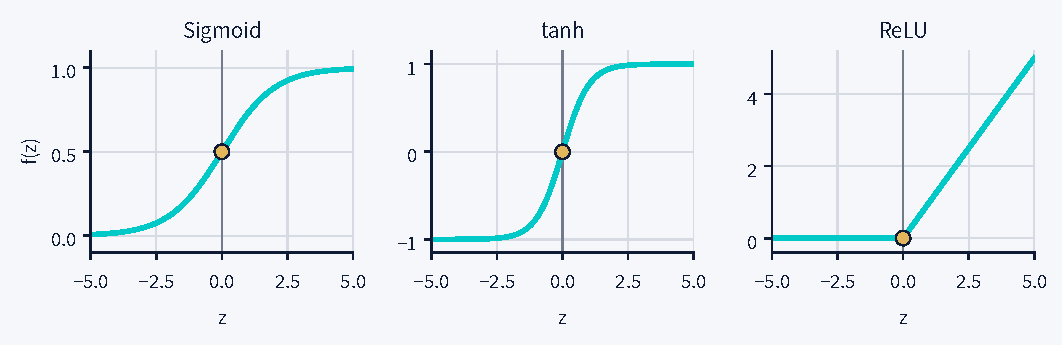
\includegraphics[width=\linewidth]{assets/charts/fig3_1_activations.pdf}
\caption{שלוש פונקציות הפעלה}\label{fig:3.1}
\figurenote{מקור: חישוב מהנוסחאות שב-\cite{S-ch03-01} (אין נתונים אמפיריים)}
\end{figure}
\begin{conceptbox}{פונקציית הפעלה}
פונקציית הפעלה (activation function) היא הכלל שקובע מה יוצא מנוירון בהינתן הסכום המשוקלל שלו. יש לה גם פרשנות ביולוגית: במודל של CS231n היא ממדלת את קצב הירי של הנוירון, כלומר באיזו תדירות הוא שולח אותות \cite{S-ch03-01}.
לאימון דרוש לה גם שיפוע מוגדר. אצל ReLU קבעו נאיר והינטון שהשיפוע הוא 0 כשהקלט קטן מאפס או שווה לו, ו-1 כשהוא חיובי, והתעלמו מהשבר שבנקודה 0 עצמה \cite{S-ch03-02}.
\end{conceptbox}
\section{משכבה לשכבה}
כבר נוירון אחד לבדו מסוגל לחזות. אם מפרשים את הפלט של נוירון עם סיגמואיד כהסתברות שדוגמה שייכת לאחת משתי קבוצות, ומאמנים אותו בהתאם, מתקבל מסווג בינארי, שמוכר גם בשם רגרסיה לוגיסטית (logistic regression) \cite{S-ch03-01}. כאן, לראשונה, מספרים הופכים לתחזית.
אבל הכוח האמיתי טמון בחיבור. ברשת נוירונים הנוירונים מסודרים בשכבות ומקושרים בגרף שאין בו מעגלים, כך שהמידע זורם קדימה ואינו חוזר אל עצמו \cite{S-ch03-01}. בשכבה מחוברת במלואה (fully-connected) כל נוירון מקושר לכל נוירון בשכבה הסמוכה, ואילו בין נוירונים באותה שכבה אין קשר בכלל \cite{S-ch03-01}. הפלט a של כל נוירון הופך לאחד הקלטים x של השכבה הבאה. השכבות שבין הקלט לפלט נקראות שכבות חבויות (hidden layers), ולשכבת הפלט בדרך כלל אין פונקציית הפעלה \cite{S-ch03-01}. ובספירה יש מוסכמה: כשאומרים "רשת בת N שכבות", לא סופרים את שכבת הקלט \cite{S-ch03-01}.
כמה פרמטרים יש בלוח כזה? חומרי הקורס עורכים חשבון: ברשת עם שלושה קלטים, שכבה חבויה של ארבעה נוירונים ושכבת פלט של שניים, יש 20 משקולות (3$\times$4 ועוד 4$\times$2) ו-6 הטיות, אחת לכל נוירון, ובסך הכול 26 פרמטרים נלמדים. מוסיפים שכבה חבויה שנייה של ארבעה ומצמצמים את הפלט לנוירון יחיד, וכבר יש 32 משקולות (3$\times$4, ועוד 4$\times$4, ועוד 4$\times$1) ו-9 הטיות, כלומר 41 \cite{S-ch03-01}. רשת זעירה, עשרות משקולות. וכשמערימים שכבות רבות, כל שכבה בונה את התיאור שלה מתוך התיאור של קודמתה \cite{S-ch01-05}, ומספר הפרמטרים מטפס במהירות.
\begin{figure}[htbp]
\centering
% Figure 3.2: one neuron and a small 3-4-2 network (structure and parameter count after S-ch03-01).
\begin{bookdiagram}[x=1cm,y=1cm]
  \tikzset{io/.style={circle,draw=turquoise,line width=0.9pt,fill=white,minimum size=8mm,inner sep=0pt}}
  % single neuron, read left to right like the formula
  \node[io] (x1) at (0,1.6) {$x_1$};
  \node[io] (x2) at (0,0.6) {$x_2$};
  \node at (0,-0.25) {$\vdots$};
  \node[io] (xn) at (0,-1.2) {$x_n$};
  \node[circle,draw=midnight,line width=1.2pt,fill=white,minimum size=11mm,font=\Large] (sum) at (4,0.2) {$\Sigma$};
  \draw[flow] (x1) -- node[above,sloped,font=\footnotesize] {$w_1$} (sum);
  \draw[flow] (x2) -- node[above,sloped,font=\footnotesize] {$w_2$} (sum);
  \draw[flow] (xn) -- node[below,sloped,font=\footnotesize] {$w_n$} (sum);
  \node[draw=gold,line width=1pt,rounded corners=1mm,fill=white,inner sep=1.5mm] (b) at (4,2.0) {הטיה $b$};
  \draw[flow] (b) -- (sum);
  \node[blk,minimum width=13mm,minimum height=10mm] (f) at (6.6,0.2) {$f$};
  \draw[flow] (sum) -- node[above] {$z$} (f);
  \node[io] (a) at (9,0.2) {$a$};
  \draw[flow] (f) -- (a);
  \node[font=\footnotesize,anchor=north] at (6.6,-0.5) {פונקציית הפעלה};
  \node[font=\footnotesize,anchor=north] at (9,-0.5) {פלט};
  \node[font=\footnotesize,anchor=north] at (0,-1.75) {קלטים};
  % small network 3 -> 4 -> 2
  \begin{scope}[yshift=-5.4cm]
    \foreach \j in {1,2,3}{\node[circle,draw=turquoise,line width=0.9pt,fill=white,minimum size=6.5mm] (i\j) at (1.5,{1.15-0.9*(\j-1)}) {};}
    \foreach \j in {1,2,3,4}{\node[circle,draw=violet,line width=0.9pt,fill=violet!22,minimum size=6.5mm] (h\j) at (4.2,{1.6-0.9*(\j-1)}) {};}
    \foreach \j in {1,2}{\node[circle,draw=turquoise,line width=0.9pt,fill=white,minimum size=6.5mm] (o\j) at (6.9,{0.7-0.9*(\j-1)}) {};}
    \foreach \p in {1,2,3}{\foreach \q in {1,2,3,4}{\draw[turquoise,line width=0.6pt] (i\p) -- (h\q);}}
    \foreach \p in {1,2,3,4}{\foreach \q in {1,2}{\draw[turquoise,line width=0.6pt] (h\p) -- (o\q);}}
    \node[font=\footnotesize] at (1.5,-1.75) {שכבת קלט};
    \node[font=\footnotesize] at (4.2,-1.75) {שכבה חבויה};
    \node[font=\footnotesize] at (6.9,-1.75) {שכבת פלט};
    \node[draw=gold,line width=1.2pt,rounded corners=1.5mm,fill=white,inner sep=2mm,align=center,font=\headingfont] at (10.0,0.25)
      {20 משקולות + 6 הטיות\\= 26 פרמטרים};
  \end{scope}
\end{bookdiagram}

\caption{נוירון אחד ורשת קטנה}\label{fig:3.2}
\figurenote{מקור: מסגרת הספר; מבנה הרשת וספירת הפרמטרים לפי \cite{S-ch03-01}}
\end{figure}
\section{מה נשאר מהמוח}
השם "נוירון" לא נבחר במקרה, ורשימות הקורס של סטנפורד אכן מקדישות סעיף להשראה הביולוגית. הנוירון הוא יחידת החישוב הבסיסית של המוח: הוא קולט אותות דרך הדנדריטים ושולח אות דרך אקסון יחיד, והמשקולות מקבילות לעוצמת הסינפסות \cite{S-ch03-01}. הערכה שמצוטטת שם מדברת על כ-86 מיליארד נוירונים במערכת העצבים של האדם, המחוברים בכ-10\textasciicircum{}14 עד 10\textasciicircum{}15 סינפסות \cite{S-ch03-01}.
גם כמה ציוני דרך מוקדמים בתולדות התחום נושאים את הזיקה למוח כבר בכותרתם. ב-1943 פרסמו מקאלוק ופיטס (Warren S. McCulloch, Walter Pitts) מאמר ששמו מדבר על "פעילות עצבית": "A logical calculus of the ideas immanent in nervous activity" \cite{S-ch03-04}. ב-1958 פרסם פרנק רוזנבלט ב-Psychological Review את "The perceptron", שכותרתו מציגה אותו כמודל הסתברותי לאחסון ולארגון של מידע במוח \cite{S-ch03-03}.
אבל אותו מדריך ממהר גם להזהיר: המודל הזה של נוירון ביולוגי גס מאוד \cite{S-ch03-01}.
\begin{mythbox}
\mythlabel רשת נוירונים היא מוח דיגיטלי קטן, והנוירונים שלה פועלים כמו אלה שבראשנו.
\tcblower
\realitylabel צוות הקורס בסטנפורד מונה ארבעה פערים לפחות \cite{S-ch03-01}. במוח יש סוגים רבים של נוירונים, שונים זה מזה בתכונותיהם. הדנדריטים לבדם מבצעים חישובים לא-ליניאריים מורכבים. סינפסה אינה מספר יחיד, אלא מערכת דינמית מסובכת. ובמערכות רבות התזמון המדויק של כל פולס חשמלי חשוב, בעוד שהמודל המלאכותי מסתפק בקצב. המדריך אף מציע להסביר רשתות נוירונים בלי שום השוואה למוח, ומזהיר שמי שיש לו רקע במדעי המוח עלול להיאנח למשמע השוואות כאלה \cite{S-ch03-01}.
\end{mythbox}
הנוירון של הספר הוא אפוא קריקטורה מתמטית מוצלחת: ההשראה שאולה מהביולוגיה, אבל הנאמנות שמורה לחשבון.
\section{בחזרה אל השאלה}
עכשיו אפשר לשוב אל הקוראת. היא עדיין עומדת ליד השיש ומביטה במסך, ואינה רואה דבר ממה שמתרחש מאחוריו. השאלה שלה, שהומרה למספרים, עוברת שכבה אחר שכבה. בכל נוירון אותו טקס קטן: מכפלות, סכום, הטיה, ברז. אף שלב בדרך לא יודע שמדובר בבצק, ואף משקולת לא "מבינה" מה היא שוקלת. ובכל זאת, בקצה השני של המערכת מתחילות להופיע מילים, אחת אחרי השנייה.
איך מודל שפה שלם הופך את זרם המספרים הזה לתשובה, מילה אחר מילה? לשם נמשיך בפרק 4.
\begin{insightsbox}
\begin{itemize}
\item נוירון מלאכותי עושה שלושה דברים פשוטים: מכפיל קלטים במשקולות, מוסיף הטיה ומעביר את הסכום דרך פונקציה לא-ליניארית \cite{S-ch03-01}.
\item המשקולות וההטיות הן הכפתורים שהאימון מכוונן \cite{S-ch03-01,S-ch01-05}. בתוך המכונה אין "בצק", יש רק מספרים כאלה.
\item פונקציית ההפעלה מכריעה כמה מהסכום עובר הלאה, והבחירה בה משפיעה על מהירות האימון ועל יציבותו \cite{S-ch03-01}.
\item השכבות הופכות יחידות זעירות למבנה שבונה תיאור על גבי תיאור, ומספר הפרמטרים גדל עם כל שכבה \cite{S-ch03-01,S-ch01-05}.
\item ההשראה ביולוגית, אבל הדמיון גס: רשת נוירונים היא מודל מתמטי, לא העתק של מוח \cite{S-ch03-01}.
\end{itemize}
\end{insightsbox}

% Generated by scripts/txt2tex.py from chapters/chapter_04.txt. Edit the TXT, not this file.
\chapterquestion{איך נולדת תשובה שלמה, אם המכונה כותבת אותה חתיכה אחר חתיכה ואינה יודעת מראש איך היא תסתיים?}
\chapter{כיצד מודל שפה מייצר תשובה}\label{ch:04}
\section{הסצנה בהילוך איטי}
חזרו אל המטבח של הקוראת. השאלה "למה הבצק שלי לא תופח, ומה אפשר לעשות עכשיו?" כבר נשלחה, ובתוך המכונה היא הפכה, כפי שראינו בפרק הקודם, לזרם של מספרים. עכשיו מתחילה התשובה לזרום: מילה מופיעה על המסך, ועוד אחת, ועוד אחת, בקצב שמזכיר מישהו שמקליד בצד השני של הקו.
נאט את הסצנה עד כמעט עצירה. דמיינו שהתשובה נפתחת, למשל, במילים "יש כמה סיבות אפשריות", משפט שהספר בחר לשם ההדגמה. בשבריר השנייה שבין "יש" לבין "כמה" המערכת לא שלפה משפט מוכן ממגירה. היא עשתה דבר צנוע יותר, ומפתיע יותר: ניחשה מה בא עכשיו.
כולנו עושים זאת בשיחה. חבר אומר "נתראה מחר ב...", ועוד לפני שסיים צצות בראש כמה השלמות, חלקן סבירות יותר מאחרות. מודל שפה (language model) הפך את ההרגל הזה לשיטה. בניסוח המתמטי, ההסתברות של טקסט שלם מתפרקת לשרשרת של שאלות קטנות, וכל אחת מהן שואלת: מה הסיכוי ליחידה הבאה, בהינתן כל מה שכבר נכתב \cite{S-ch04-03,S-ch04-04}. כך נוצר הטקסט, מתחילתו לסופו, יחידה אחר יחידה \cite{S-ch04-03}. נעקוב אחרי המילה "כמה" מרגע שהשאלה התקבלה ועד שהופיעה על המסך.
\section{לקבל את הטקסט, ולפרק אותו}
השלב הראשון נשמע מובן מאליו: לקבל את הטקסט כמו שהוא. אבל זו החלטה. מחברי הדוח על GPT-2 (2019) מתארים עיבוד מקדים שמקובל במודלי שפה, כמו המרת כל האותיות לאותיות קטנות, שמגביל את המחרוזות שהמודל מסוגל לייצג. את GPT-2 הם תכננו כך שיוותר על עיבוד שמאבד מידע, ויוכל להעניק הסתברות לכל מחרוזת Unicode \cite{S-ch04-04}.
עכשיו צריך לפרק את הטקסט ליחידות. למה לא פשוט למילים? כי אוצר מילים שלם הוא עצום, וכל מילה שלא הופיעה בו הופכת לסימן כללי של "לא ידוע". ואם נפרק לאותיות בודדות, הרצפים מתארכים מאוד, ואות אחת נושאת הרבה פחות משמעות ממילה שלמה \cite{S-ch04-06}. שפה היא בעיה פתוחה, שבה תמיד צצות מילים חדשות, בעוד שאוצר המילים של מודלי תרגום נוירוניים הוגבל בדרך כלל, נכון ל-2016, ל-30,000 עד 50,000 מילים \cite{S-ch04-02}.
הפתרון הוא דרך ביניים: חלקי מילים (subword units). מילה נפוצה נשארת יחידה אחת, ומילה נדירה מתפרקת לחלקים \cite{S-ch04-06}. סנריך ועמיתיו התאימו ב-2016 לפירוק כזה את שיטת קידוד זוגות הבתים (Byte Pair Encoding, BPE): מתחילים מתווים בודדים, מוצאים את זוג הסמלים הסמוכים השכיח ביותר, ממזגים אותו לסמל חדש, וחוזרים חלילה. מספר המיזוגים הוא ההגדרה היחידה שצריך לבחור \cite{S-ch04-02}. בדוגמה מהמאמר, המילה lower, שלא הופיעה במילון שממנו נלמדו המיזוגים, פורקה ל-low ול-er \cite{S-ch04-02}.
ב-GPT-2 הרעיון הזה מופעל על בתים במקום על אותיות, ולכן האוסף הבסיסי שלו מונה רק 256 סמלים \cite{S-ch04-04}. אוצר המילים המלא שלו מונה 50,257 טוקנים: 256 בתים, 50,000 מיזוגים וטוקן מיוחד אחד שמסמן סוף טקסט \cite{S-ch04-06}.
ומה קורה למילה "תופח" מהשאלה של הקוראת? ייתכן שהיא תישאר שלמה, וייתכן שתתפרק, נניח, ל"תופ" ול"ח". זה פירוק להמחשה בלבד: הספר לא בדק טוקנייזר מסוים על עברית, והפירוק בפועל תלוי באוצר המילים של כל מערכת.
\begin{conceptbox}{טוקן (token)}
טוקן הוא יחידת הטקסט הבסיסית שמודל שפה קורא וכותב. הוא יכול להיות מילה שלמה, חלק ממילה, תו או בית, לפי אוצר המילים של הטוקנייזר \cite{S-ch04-06}. אוצר המילים הוא רשימה סגורה: ב-GPT הראשון היו בה 40,478 טוקנים, וב-GPT-2 50,257 \cite{S-ch04-06}. לכל טוקן ברשימה יש מספר סידורי.
פרט שקל לפספס: המודל סופר טוקנים, לא מילים. חלון ההקשר של GPT-2, כלומר כמות הטקסט שהוא מסוגל להביא בחשבון בבת אחת, מוגדר ב-1,024 טוקנים \cite{S-ch04-04}.
\end{conceptbox}
\section{כתובת במרחב של משמעויות}
מספר סידורי ברשימה עדיין אינו משמעות. ב-2013 תיארו מיקולוב ועמיתיו את המצב שהיה נפוץ אז: מערכות רבות התייחסו למילים כאל יחידות אטומיות, אינדקסים באוצר מילים בלי שום מושג של דמיון ביניהם \cite{S-ch04-05}. מבחינתן, "בצק" רחוקה מ"עיסה" בדיוק כמו מ"מטרייה".
החלופה היא לייצג כל מילה כווקטור, כלומר כרשימה ארוכה של מספרים, כך שמילים דומות נוטות להיות קרובות זו לזו במרחב, ויכולות להיות ביניהן כמה דרגות של דמיון \cite{S-ch04-05}. מיקולוב ועמיתיו הציעו דרך יעילה ללמוד וקטורים כאלה מאוסף עצום של טקסט \cite{S-ch04-05}. המאמר מביא מעבודה קודמת דוגמה שנעשתה מפורסמת: אם לוקחים את הווקטור של King, מחסירים ממנו את הווקטור של Man ומוסיפים את זה של Woman, הווקטור הקרוב ביותר לתוצאה הוא זה של Queen \cite{S-ch04-05}. משמעות הופכת לגאומטריה.
לייצוג כזה קוראים שיבוץ (embedding). ב-Transformer, הארכיטקטורה שעליה נשענים מודלי השפה בפרק הזה, כל טוקן מקבל וקטור נלמד, שבמאמר המקורי משנת 2017 אורכו 512 מספרים \cite{S-ch04-01}. הווקטורים האלה נלמדים יחד עם המודל כולו \cite{S-ch04-01}, ומיד אחר כך עוברים שלב שמערב בהם מידע מהמילים שמסביב.
\section{להקשיב למילים הנכונות}
בשאלה של הקוראת, "עכשיו" נקשרת ל"לעשות", ו"שלי" נקשרת ל"בצק". כדי להבין מילה צריך לדעת למי מהשכנות שלה להקשיב. על זה בדיוק מופקד מנגנון הקשב (attention).
המאמר "Attention Is All You Need" (2017) הציג ארכיטקטורה שמוותרת על רקורסיה (recurrence), כלומר על מעבר על הקלט מילה אחר מילה בתוך הרשת, ונשענת כולה על קשב \cite{S-ch04-01}. כל מיקום ברצף שולח מעין שאילתה (query). כל מיקום, כולל השולח עצמו, מציע מפתח (key), שמתאר במה הוא יכול לעזור, וערך (value), שהוא התוכן שהוא מוסר. הפלט הוא סכום משוקלל של הערכים: ככל שהשאילתה מתאימה יותר למפתח, כך המשקל של הערך גבוה יותר \cite{S-ch04-01}. במאמר פועלים במקביל שמונה "ראשי" קשב, וכל אחד מהם יכול להתמקד בקשר אחר \cite{S-ch04-01}.
עוד כלל אחד חשוב לסצנה שלנו: בזמן הכתיבה, כל מיקום רשאי לפנות רק אל מה שלפניו \cite{S-ch04-01}. המודל לא מציץ במילים שעוד לא נכתבו, ממש כמו שאי אפשר לשמוע את סוף המשפט של החבר לפני שאמר אותו.
\section{ציון לכל טוקן, הסתברות לכל המשך}
בסוף העיבוד, טרנספורמציה לינארית נלמדת מעניקה ציון לכל אחד מהטוקנים באוצר המילים, ופונקציה בשם softmax הופכת את הציונים להסתברויות לטוקן הבא \cite{S-ch04-01}. הולצמן ועמיתיו קוראים לציונים האלה logits \cite{S-ch04-03}.
בחזרה לרגע שאחרי "יש". דמיינו שההסתברויות נראות כך: "כמה" 0.46, "מספר" 0.22, "סיבות" 0.12, "לא" 0.05, וכל שאר אוצר המילים חולק את היתר. מספרים להמחשה בלבד.
ההתפלגות הזאת לא תמיד נראית אותו דבר. הולצמן ועמיתיו מראים שלפעמים היא שטוחה, עם המון המשכים סבירים, כמו אחרי פתיחה של ציטוט, ולפעמים מחודדת: אחרי "I ate the pizza while it was still" כמעט כל ההסתברות מרוכזת במילה אחת, "hot" \cite{S-ch04-03}.
\section{הרגע שבו נבחרת מילה}
הסתברויות אינן החלטה. את ההחלטה מקבלת אסטרטגיית פענוח (decoding strategy), כלל שקובע איך בוחרים את הטוקן הבא \cite{S-ch04-07}, והכלל הזה לבדו יכול לשנות מאוד את איכות הטקסט שמפיק אותו מודל \cite{S-ch04-03}.
הדרך הפשוטה היא בחירה חמדנית (greedy): בכל שלב לוקחים את הטוקן הסביר ביותר. בספריית Transformers של Hugging Face זו ברירת המחדל, והיא מתאימה לפלטים קצרים, אבל בטקסט ארוך היא מתחילה לחזור על עצמה \cite{S-ch04-07}. חיפוש אלומה (beam search) עוקב אחרי כמה רצפים במקביל ובוחר את זה שההסתברות הכוללת שלו הגבוהה ביותר \cite{S-ch04-07}. אלא שלפי הולצמן ועמיתיו, ניסיון למקסם הסתברות מוביל לטקסט תפל, לא קוהרנטי, או כזה שנתקע בלולאות של חזרות \cite{S-ch04-03}.
החלופה היא דגימה (sampling): הגרלה לפי ההתפלגות, שבה לכל טוקן שההסתברות שלו אינה אפס יש סיכוי להיבחר, ולכן פחות חזרות ויותר גיוון \cite{S-ch04-07}. אבל דגימה טהורה עלולה להפיק גיבוב, כפי שהולצמן ועמיתיו הדגימו על GPT-2 \cite{S-ch04-03}. דרכי הביניים מצמצמות את ההגרלה: ב-top-k מגרילים רק מתוך k הטוקנים הסבירים ביותר, וב-top-p, שנקראת גם דגימת גרעין (nucleus), מגרילים מתוך הקבוצה הקטנה ביותר שההסתברויות שלה מצטברות לפחות ל-p. גודל הקבוצה משתנה בכל הגרלה לפי צורת ההתפלגות \cite{S-ch04-03}.
הגדרה נוספת היא הטמפרטורה (temperature): מחלקים את הציונים במספר t לפני ה-softmax. ערך קטן מ-1 מטה את ההתפלגות לטובת הטוקנים הסבירים, והורדת הטמפרטורה משפרת את האיכות במחיר של פחות גיוון \cite{S-ch04-03}. כאן "טמפרטורה" היא פרמטר כוונון של הדגימה. בפרק 6 נפגוש את אותה מילה במשמעות אחרת, ואסור לבלבל ביניהן.
\begin{figure}[htbp]
\centering
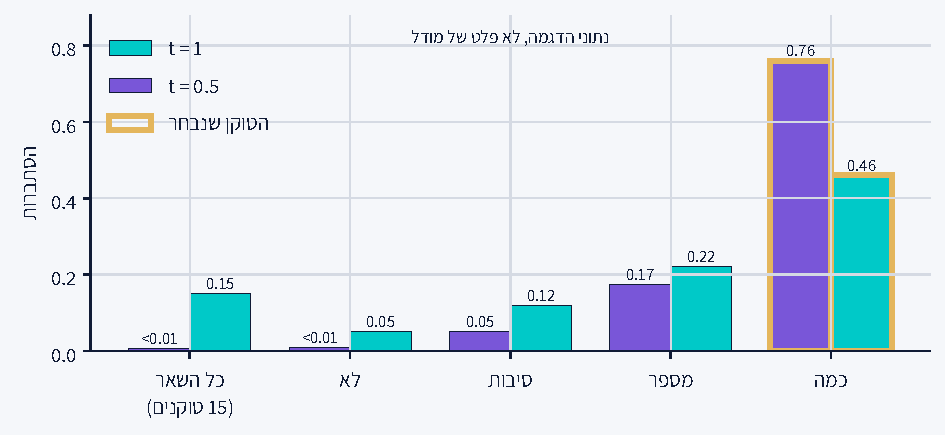
\includegraphics[width=\linewidth]{assets/charts/fig4_1_temperature.pdf}
\caption{אותם ציונים, שתי טמפרטורות}\label{fig:4.1}
\figurenote{נתוני הדגמה, לא פלט של מודל · מקור: נתוני הדגמה (ציונים מומצאים); הנוסחה מ-\cite{S-ch04-03}}
\end{figure}
\begin{behindbox}{הלולאה, טוקן אחר טוקן}
המפענח ב-Transformer הוא אוטו-רגרסיבי: הוא מייצר סמל אחד בכל פעם, וכל סמל שכבר נוצר נכנס כקלט ליצירת הסמל הבא \cite{S-ch04-01}. בתיעוד של Hugging Face הלולאה נראית בקוד כמעט כפי שהיא: מחשבים ציונים, בוחרים את הגבוה שבהם, מצרפים את הטוקן שנבחר לקלט וחוזרים על הכול \cite{S-ch04-07}.
בסצנה שלנו: "יש" נבחרה ונוספה לסוף הרצף. כל הרצף, השאלה ו"יש", עובר שוב את הדרך, ורק אז מופיעה "כמה". כך הלאה, עד סוף התשובה. גם GPT-3 מתואר על ידי מפתחיו כמודל שפה אוטו-רגרסיבי \cite{S-ch04-08}.
\end{behindbox}
\section{תשעה צעדים, ותרשים שמודה בפשטותו}
\begin{figure}[htbp]
\centering
% Figure 4.2: from the question to the answer in nine steps (9 block nodes + generation loop).
% Read right to left, snaking down; block 8 ("בחירת טוקן") is highlighted in Gold.
\begin{bookdiagram}[x=1cm,y=1cm]
  \tikzset{st/.style={blk,text width=3.6cm,minimum height=12mm}}
  \node[st] (s1) at (12.2,0)    {שאלת משתמש};
  \node[st] (s2) at (7.1,0)     {קבלת הטקסט};
  \node[st] (s3) at (2.0,0)     {פירוק לטוקנים};
  \node[st] (s4) at (2.0,-2.3)  {ייצוג מספרי};
  \node[st] (s5) at (7.1,-2.3)  {עיבוד קשב};
  \node[st] (s6) at (12.2,-2.3) {חישוב ציוני טוקנים};
  \node[st] (s7) at (12.2,-4.6) {המרה להסתברויות};
  \node[st,draw=gold,line width=2.2pt] (s8) at (7.1,-4.6) {בחירת טוקן};
  \node[st] (s9) at (2.0,-4.6)  {הרכבת תשובה};
  \foreach \n in {1,...,9}{\node[num] at ($(s\n.north east)+(-0.08,-0.08)$) {\n};}
  \foreach \a/\b in {1/2,2/3,3/4,4/5,5/6,6/7,7/8,8/9}{\draw[flow] (s\a) -- (s\b);}
  \draw[loop,solid,line width=1.4pt] (s8.south) -- ++(0,-0.8) -| ($(s4.west)+(-0.7,0)$) -- (s4.west);
  \node[font=\footnotesize\headingfont,text=violet] at (7.1,-5.75) {הטוקן שנבחר מצטרף לרצף, והלולאה חוזרת};
\end{bookdiagram}

\caption{מהשאלה אל התשובה, בתשעה צעדים}\label{fig:4.2}
\figurenote{תרשים הסברתי ומפושט, לא ארכיטקטורה מלאה · מקור: מסגרת הספר, על בסיס \cite{S-ch04-01}, \cite{S-ch04-03}, \cite{S-ch04-04} ו-\cite{S-ch04-07}}
\end{figure}
התרשים הזה מוותר על פרטים רבים כדי שאפשר יהיה לראות משהו: הוא הסבר מפושט, ולא תיאור מלא של ארכיטקטורת מודל. ב-Transformer המקורי מתווסף לכל וקטור, פעם אחת בכניסה, קידוד של מיקומו ברצף. שכבות הקשב, ולצידן שכבות עיבוד שאינן קשב, מוערמות שש פעמים זו על גבי זו \cite{S-ch04-01}. המודל המקורי נבנה לתרגום מכונה, משני חלקים, מקודד ומפענח \cite{S-ch04-01}, ו-GPT-2 מבוסס על הארכיטקטורה הזאת בשינויים \cite{S-ch04-04}.
גם קנה המידה נעלם מהתרשים: הגרסה הגדולה של GPT-2 כוללת 1.5 מיליארד פרמטרים \cite{S-ch04-04}, ו-GPT-3, שהוצג ב-2020, כולל 175 מיליארד \cite{S-ch04-08}. במה שמוצרים מסחריים מוסיפים סביב המודל הספר אינו עוסק. ולבסוף, הבלוקים נראים כמו תהליך שרץ פעם אחת, בעוד שבפועל רובם חוזרים לכל טוקן חדש. זה תפקידו של חץ הלולאה.
\begin{thinkbox}
אם הקוראת תשאל את אותה שאלה פעמיים, בדיוק באותן מילים, ותקבל שתי תשובות בניסוח שונה, איזו מהן היא "התשובה של המערכת"? ואם טמפרטורה נמוכה הופכת את התשובות לדומות יותר זו לזו, האם היא גם הופכת אותן לנכונות יותר? מה בדיוק הייתם רוצים למדוד כדי לדעת?
\end{thinkbox}
\section{התשובה שעל המסך}
כעבור כמה שניות מסתיימת התשובה. הקוראת רואה פסקה רהוטה, שלמה, כאילו נכתבה במחשבה תחילה. עכשיו אנחנו יודעים שהיא נבנתה ניחוש אחר ניחוש, וכל מילה בה נבחרה מתוך התפלגות. רהיטות היא תוצר של הסתברויות, לא הוכחה לאמת.
וכאן עולה השאלה הבאה, זו שהקוראת עצמה כבר מתחילה לשאול: איך יודעים אם תשובה כזאת טובה? על כך בפרק הבא.
\begin{insightsbox}
\begin{itemize}
\item מודל שפה אינו שולף תשובות מוכנות. הוא מנחש בכל צעד את הקטע הבא של הטקסט, על סמך כל מה שנכתב עד אז \cite{S-ch04-03,S-ch04-04}.
\item הטוקן, ולא המילה, הוא יחידת העבודה. שיטות כמו BPE מאפשרות לייצג גם מילה שהמערכת מעולם לא ראתה, באמצעות חלקים מוכרים \cite{S-ch04-02,S-ch04-06}.
\item שיבוצים הופכים מספר סידורי למיקום במרחב, וקשב מאפשר לכל מיקום ברצף לשקלל מידע מהמיקומים האחרים \cite{S-ch04-01,S-ch04-05}.
\item אותן הסתברויות יכולות להוליד טקסטים שונים מאוד: הבחירה בין חמדנות, חיפוש אלומה, דגימה וטמפרטורה משנה את התוצאה \cite{S-ch04-03,S-ch04-07}.
\item כל תרשים של התהליך הוא פישוט. מה שחשוב לזכור ממנו הוא הלולאה: כל מילה שנבחרה הופכת לחלק מהקלט של המילה הבאה \cite{S-ch04-01}.
\end{itemize}
\end{insightsbox}

% Generated by scripts/txt2tex.py from chapters/chapter_05.txt. Edit the TXT, not this file.
\chapterlayout{05}
\chapterquestion{איך יודעים שמכונה באמת למדה, ולא רק נשמעת כאילו למדה?}
\chapter{בודקים מודלים בעזרת נתונים}\label{ch:05}
\section{השאלה שאחרי התשובה}
התשובה על הבצק כבר ממלאת את המסך. היא מסודרת בסעיפים, מנוסחת בביטחון, ואפילו מציעה מה לעשות עכשיו. אבל אחרי הקריאה הראשונה הקוראת נעצרת מול שאלה שקטה יותר: איך אני יודעת שזה נכון? ומי בדק את המערכת הזאת לפני שהגיעה אליי?
את מודל השפה שענה לה הספר לא יכול לפרק ולבחון. אבל אפשר להראות מקרוב את העיקרון שעליו נשענת בדיקה של מערכת לומדת: לא שואלים אותה על מה שכבר ראתה. מודל טוב הוא מודל שמנבא היטב גם על נתונים חדשים, ולתכונה הזאת קוראים הכללה (generalization) \cite{S-ch05-08}. כדי למדוד אותה מציבים מול המכונה דוגמאות שלא פגשה מעולם, ומונים כמה פעמים צדקה.
וזה מה שנעשה בפרק הזה, ובסופו הספר יריץ ניסוי משלו.
\section{לספור פגיעות}
המדד הפשוט ביותר נקרא דיוק (accuracy): החלק היחסי של התחזיות שתואמות את התשובה האמיתית \cite{S-ch05-01}. התיעוד של ספריית scikit-learn מביא דוגמה זעירה: ארבע דוגמאות שהתוויות האמיתיות שלהן הן 0, 1, 2 ו-3, ומודל שעונה 0, 2, 1 ו-3. שתי תשובות נכונות מתוך ארבע, כלומר דיוק של 0.5 \cite{S-ch05-01}.
\begin{conceptbox}{דיוק ושיעור שגיאה}
בפרק 1 פגשנו מסנן דואר זבל, ואת מדד הביצוע שלו: החלק של ההודעות שסווגו נכון. למדד הזה יש שם. כל הודעה מסתיימת באחת מארבע תוצאות: זבל שהגיע לתיקיית הזבל (חיובי אמיתי, TP), הודעה תקינה שנשלחה לשם בטעות (חיובי שגוי, FP), זבל שחמק לתיבה הנכנסת (שלילי שגוי, FN), והודעה תקינה שהגיעה למקומה (שלילי אמיתי, TN) \cite{S-ch05-07}.
\begin{equation}
\text{Accuracy} = \frac{TP + TN}{TP + TN + FP + FN}
\end{equation}
במונה: שתי ההחלטות הנכונות. במכנה: כל ההודעות \cite{S-ch05-06}.
שיעור השגיאה (error rate) הוא המשלים: שיעור השגיאה = 1 פחות הדיוק.
\end{conceptbox}
מספר אחד נוח לזכור, אבל הוא גם נוח להסתיר. חומרי הלימוד של Google מציגים מקרה מאלף: אם מחלקה מסוימת מופיעה רק באחוז אחד מהמקרים, מודל שעונה תמיד "לא" יקבל דיוק של 99\%, ובכל זאת אין בו שום תועלת \cite{S-ch05-06}. כשהנתונים לא מאוזנים, או כשסוג אחד של טעות יקר מהשני, עדיף להיעזר במדדים שמסתכלים על כל סוג טעות בנפרד \cite{S-ch05-06}.
\section{שני סוגים של טעות}
שני מדדים כאלה שווה להכיר בשמם. הראשון הוא דייקנות (precision): מתוך כל מה שהמסווג סימן כחיובי, כמה היה חיובי באמת. לפי תיעוד scikit-learn, זו היכולת שלו לא לתייג דוגמה שלילית כחיובית \cite{S-ch05-01}. השני הוא כיסוי (recall): מתוך כל הדוגמאות החיוביות שהיו שם, כמה הוא הצליח למצוא \cite{S-ch05-01}. בשפת ארבע התוצאות, הדייקנות היא TP חלקי סכום TP ו-FP, והכיסוי הוא TP חלקי סכום TP ו-FN \cite{S-ch05-06}. במסנן הדואר, דייקנות נמוכה פירושה הודעות תקינות שנבלעות בתיקיית הזבל, וכיסוי נמוך פירושו זבל שממשיך להציף את התיבה.
אותו תיעוד מביא דוגמה קטנה שאפשר לחשב ביד: שמונה דוגמאות, שלוש שליליות וחמש חיוביות. מתוך שלוש השליליות המסווג זיהה נכון שתיים וטעה באחת (TN=2, FP=1), ומתוך חמש החיוביות מצא שלוש והחמיץ שתיים (TP=3, FN=2) \cite{S-ch05-01}. הדיוק הוא 5 מתוך 8, כלומר 0.625, ושיעור השגיאה 0.375. הדייקנות היא 3 מתוך 4, כלומר 0.75, והכיסוי 3 מתוך 5, כלומר 0.6.
\begin{table}[htbp]
\centering
\caption{מדדים במבט אחד}\label{tab:5.1}
\begingroup\small\renewcommand{\arraystretch}{1.35}\booktablerule
\begin{tabularx}{\linewidth}{RRRR}
\toprule
\rowcolor{midnight}\tabhead{מדד} & \tabhead{השאלה שהוא עונה עליה} & \tabhead{נוסחה} & \tabhead{מה נעלם ממנו}\\ \midrule
דיוק (accuracy) & באיזה חלק מכל המקרים המודל צדק? & (TP+TN) / (TP+TN+FP+FN) \cite{S-ch05-06} & כשמחלקה נדירה, גם מודל חסר תועלת מציג דיוק גבוה \cite{S-ch05-06}\\
שיעור שגיאה (error rate) & באיזה חלק מהמקרים המודל טעה? & 1 פחות הדיוק (נגזר מהנוסחה) & אותה חולשה כמו הדיוק, כי זה אותו מידע בהיפוך\\
דייקנות (precision) & מתוך מה שסומן כחיובי, כמה חיובי באמת? & TP / (TP+FP) \cite{S-ch05-06} & החיוביים שהוחמצו: הנוסחה אינה כוללת את FN\\
כיסוי (recall) & מתוך החיוביים שהיו, כמה נמצאו? & TP / (TP+FN) \cite{S-ch05-06} & התרעות השווא: הנוסחה אינה כוללת את FP\\
\bottomrule
\end{tabularx}
\endgroup
\end{table}
התיעוד של scikit-learn מציע גם דיוק מאוזן (balanced accuracy), שנועד למנוע הערכות מנופחות כשהמחלקות אינן מאוזנות \cite{S-ch05-01}. וסוקולובה ולפאלם (Sokolova \& Lapalme) פרסמו ב-2009 ניתוח שיטתי של מדדי ביצוע למשימות סיווג \cite{S-ch05-11}.
כאן מתחילה הערכת תוצאות (evaluation), שהיא יותר מחישוב של מספר. היא פותחת בשאלה על אילו נתונים נמדד המספר, ממשיכה בשאלה איזו טעות יקרה יותר במשימה הזאת \cite{S-ch05-06}, ורק אז בוחרת מדד. דמיינו מי שמחכה למכתב חשוב: היא תעדיף שקצת זבל יחמוק לתיבה, ובלבד שהמכתב לא ייעלם בתיקיית הזבל. בשבילה, דייקנות חשובה יותר מכיסוי. והשאלה האחרונה אינה פחות חשובה: מה המספר עלול להסתיר.
\section{שתי ערמות של דוגמאות}
נניח שמודל למד לזהות ספרות בכתב יד. אם נמדוד את הדיוק שלו על אותן דוגמאות שמהן למד, נקבל דיוק אימון. אם נמדוד על דוגמאות שהוחזקו בצד, נקבל דיוק בדיקה. רק הוא מספר משהו על ההכללה. זו החלוקה לאימון ולבדיקה שפגשנו בפרק 2. השגיאה על הדוגמאות שבצד היא אומדן של מה שבאמת מעניין אותנו: השגיאה הצפויה של המודל על נתונים חדשים \cite{S-ch05-13}. להפרש בין השגיאה הזאת לשגיאת האימון קוראים פער הכללה (generalization gap) \cite{S-ch05-12}. יש חוקרים שמכנים את הפער הזה גם שגיאת הכללה (generalization error) \cite{S-ch05-10,S-ch05-12}.
דמיינו קורא כתב יד שלא למד את צורת הספרה 4, אלא שינן כל כתם דיו וכל רעד של עט בערמה שהוצגה לו. על הערמה הזאת הוא כמעט לא טועה. כשמגיעה מעטפה מכותב חדש, הוא אובד עצות. לתופעה הזאת קוראים התאמת יתר (overfitting): מודל שתואם את קבוצת האימון (משנן אותה) עד כדי כך שהוא נכשל בחיזוי נכון על נתונים חדשים. הכללה היא ההפך שלה. ובתת-התאמה (underfitting) המודל אינו מנבא טוב אפילו על נתוני האימון \cite{S-ch05-08}.
תיעוד scikit-learn מציע כלל אצבע לקריאת עקומות, שמשווה בין ציון האימון לבין הציון על קבוצת אימות (validation set), כלומר נתונים שהמודל לא למד מהם. אם שני הציונים נמוכים, זה סימן לתת-התאמה: המודל פשוט מדי ולא תפס את הדפוס. אם ציון האימון גבוה וציון האימות נמוך, זה סימן להתאמת יתר. ומצב הפוך, ציון אימון נמוך עם ציון אימות גבוה, בדרך כלל אינו אפשרי \cite{S-ch05-02}. (בניסוי של הספר אין קבוצת אימות; ציון הבדיקה שבו משמש לדיווח בלבד.)
\begin{mythbox}
\mythlabel מודל שמגיע לדיוק כמעט מושלם על נתוני האימון הוא מודל טוב.
\tcblower
\realitylabel במאמר שהוצג בכנס ICLR ב-2017 הראו ג'אנג (Zhang) ועמיתיו שרשתות עמוקות מצליחות "ללמוד" גם תוויות שהוגרלו באקראי. שגיאת האימון מגיעה לאפס, ושגיאת הבדיקה אינה טובה מניחוש מקרי \cite{S-ch05-10}. במערך התמונות CIFAR10, מודל Inception שאומן על תוויות אקראיות הגיע ל-100.0\% דיוק אימון ול-9.78\% בלבד בבדיקה (טבלה 1 במאמר) \cite{S-ch05-10}. התמונות עצמן היו אמיתיות, אבל בינן לבין התוויות לא היה שום קשר. ובכל זאת הרשת שיננה כל אחת מהן, ורק קבוצת בדיקה נפרדת חשפה זאת.
\end{mythbox}
\section{הניסוי של הספר: ספרות בכתב יד}
בפרק 1 פגשנו את המכונות שממיינות דואר לפי ספרות שנכתבו ביד. עכשיו הספר מריץ בעצמו מודל קטן על ספרות בכתב יד, ומודד אותו כפי שתואר כאן.
הנתונים מגיעים מהמאגר שנקרא Optical Recognition of Handwritten Digits, של אלפיידין וקיינק (Alpaydin \& Kaynak), שנתרם ב-1998 למאגר UCI Machine Learning Repository ומופץ ברישיון פתוח CC BY 4.0 \cite{S-ch05-05}. המאגר המלא כולל 5,620 דוגמאות \cite{S-ch05-05}. הניסוי משתמש בעותק שמופץ עם scikit-learn תחת השם load\_digits: 1,797 תמונות של ספרות, כל אחת רשת של 8 על 8 משבצות, כלומר 64 תכונות, שבכל אחת מספר שלם בין 0 ל-16, ועשר מחלקות, הספרות 0 עד 9 \cite{S-ch05-04}. לפי התיעוד, זה עותק של קבוצת הבדיקה של המאגר המקורי \cite{S-ch05-04}.
\begin{labbox}{איך נבנה הניסוי}
\begin{enumerate}
\item טוענים את 1,797 הספרות \cite{S-ch05-04}.
\item מחלקים אותן פעם אחת: 75\% לאימון ו-25\% לבדיקה, בחלוקה מרובדת לפי ספרה. יוצאות 1,347 דוגמאות אימון ו-450 דוגמאות בדיקה. זרע אקראי (seed) קבוע, 42, מבטיח שכל הרצה חוזרת תיתן את אותה חלוקה.
\item מנרמלים את הערכים, והנרמול נלמד מקבוצת האימון בלבד, כדי שמידע מהבדיקה לא יזלוג פנימה.
\item מאמנים רשת נוירונים קטנה: שכבה חבויה אחת של 32 נוירונים, במשך 40 תקופות אימון (epochs). בסוף כל תקופה מודדים דיוק על שתי הקבוצות. דיוק הבדיקה נמדד לדיווח בלבד, ולא שימש לאימון, לנרמול או לבחירת מודל או תקופה.
\item שומרים את המספרים לקובץ CSV, ומשם מציירים את הגרף ואת הטבלה.
\end{enumerate}
כלל היושר של הניסוי: כל ההגדרות, כולל מספר התקופות, נקבעו לפני ההרצה. מציגים את מה שיצא. אם לא יופיע פער בין אימון לבדיקה, הספר יאמר זאת, ולא ישנה הגדרות עד שתופיע הצורה "הנכונה".
\end{labbox}
\begin{figure}[htbp]
\centering
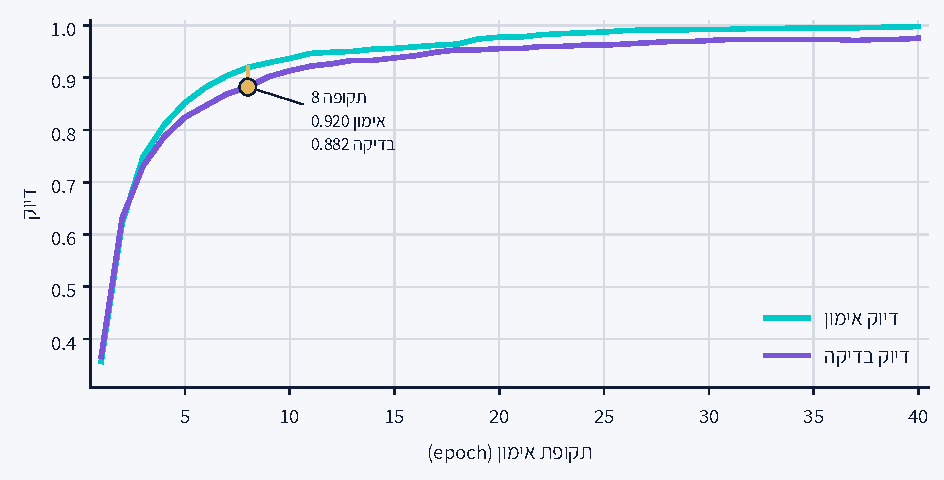
\includegraphics[width=\linewidth]{assets/charts/fig5_1_accuracy.pdf}
\caption{דיוק אימון מול דיוק בדיקה לאורך תקופות האימון}\label{fig:5.1}
\figurenote{המספרים חושבו בניסוי של הספר על נתוני UCI Digits (Alpaydin \& Kaynak, 1998, CC BY 4.0) · מקור: ניסוי M4, python/data/digits\_accuracy.csv שמופק על ידי python/generate\_chart.py}
\end{figure}
\begin{table}[htbp]
\centering
\caption{דיוק אימון ודיוק בדיקה לפי תקופת אימון (ניסוי הספר, UCI Digits)}\label{tab:5.2}
\begingroup\small\renewcommand{\arraystretch}{1.35}\booktablerule
\begin{tabular}{ccc}
\toprule
\rowcolor{midnight}\tabhead{תקופה} & \tabhead{דיוק אימון} & \tabhead{דיוק בדיקה}\\ \midrule
1 & 0.357 & 0.367\\
5 & 0.852 & 0.824\\
8 & 0.920 & 0.882\\
10 & 0.937 & 0.913\\
15 & 0.956 & 0.938\\
20 & 0.978 & 0.956\\
25 & 0.987 & 0.962\\
30 & 0.993 & 0.971\\
35 & 0.995 & 0.973\\
40 & 0.998 & 0.976\\
\bottomrule
\end{tabular}
\endgroup
\end{table}
\section{איך לקרוא את הגרף, ומה לא לקרוא בו}
אפשר לקרוא את הגרף לפי כלל האצבע, אם משאילים אותו מקבוצת אימות לקו הבדיקה (הכלל עצמו מנוסח בתיעוד לקבוצת אימות). אם שני הקווים עולים ונשארים קרובים זה לזה, המודל מכליל היטב על החלוקה הזאת. אם דיוק האימון גבוה ודיוק הבדיקה נמוך ממנו בהרבה, זה המצב שתיעוד scikit-learn מזהה עם התאמת יתר \cite{S-ch05-02}. ואם שני הקווים נשארים נמוכים, זה סימן לתת-התאמה \cite{S-ch05-02}.
יש גרפים שמציגים הפסד (loss) במקום דיוק: מספר שמודד עד כמה התחזיות רחוקות מהתשובות הנכונות, וככל שהוא נמוך יותר, טוב יותר. בעקומות כאלה הסימן המוכר הוא שהפסד האימון ממשיך לרדת בזמן שההפסד על הנתונים שהוחזקו בצד מתחיל לעלות. לפי Google, דפוס כזה מרמז בחוזקה על התאמת יתר \cite{S-ch05-08}.
מה יצא בפועל, כפי שמופיע באיור~\ref{fig:5.1} ובטבלה~\ref{tab:5.2}? שני הקווים עולים מהר עד התקופה העשירית בערך, ואחר כך מתמתנים. דיוק הבדיקה אינו מתדרדר: מלבד ירידה זעירה אחת בתקופה 37 (מ-0.973 ל-0.971, ובתקופה 38 חזרה ל-0.973) הוא מתייצב סביב 0.97 מתקופה 30. דיוק האימון ממשיך להתקרב ל-1. בסוף האימון דיוק האימון הוא 0.998 ודיוק הבדיקה 0.976, פער הכללה מוערך של 2.2 נקודות אחוז. הפער הגדול ביותר, 3.8 נקודות, היה בתקופה 8 (0.920 מול 0.882), והיא הנקודה המודגשת באיור; נבחרה לפי כלל קבוע ולא בעין. לפי כלל האצבע, זו אינה תת-התאמה, כי שני הציונים גבוהים. יש פער קטן ועקבי בין האימון לבדיקה, אבל לא הדפוס של התאמת יתר, שבו הבדיקה מתדרדרת. כדאי לא להסיק מהמספרים יותר מדי. ראשית, זו חלוקה אחת עם זרע אקראי אחד. חלוקה אחרת עשויה לתת קווים מעט שונים, ולכן הגרף מתאר את הניסוי הזה, לא חוק טבע. שנית, אם נבחר בדיעבד את התקופה "הטובה ביותר" לפי קו הבדיקה, הבדיקה כבר השפיעה על ההחלטה. ג'אנג ועמיתיו מעירים שכדי לטעון בקפדנות שעצירה מוקדמת (early stopping) משפרת הכללה, צריך קבוצת בדיקה מבודדת נוספת \cite{S-ch05-10}. שלישית, חומרי הלימוד של Google מזכירים שעקומות הפסד קשות לא פעם לפרשנות \cite{S-ch05-09}. ורביעית, מסווג קטן של ספרות בגודל 8 על 8 פיקסלים אינו מודל שפה. הניסוי מדגים שיטת בדיקה, ולא מעיד דבר על איכות התשובה שהקוראת קיבלה על הבצק.
\section{בחזרה אל המסך}
הקוראת לא תראה לעולם את קבוצת הבדיקה של המערכת שענתה לה. אבל עכשיו היא יודעת מה לשאול: על אילו נתונים נמדדה המערכת, האם אלה נתונים שלא ראתה, איזו טעות נספרה, ומה המספר מסתיר. בדיקה טובה היא תנאי הכרחי לאמון, אבל לא ערובה מלאה: גם מערכת שנבחנה היטב טועה לפעמים, ולפעמים דווקא בטון הבטוח ביותר. על הגבולות האלה, ועל מה שקורה למה שהקוראת הקלידה, נדבר בפרק 6.
\begin{insightsbox}
\begin{itemize}
\item דיוק עונה על שאלה אחת בלבד: באיזה חלק מהמקרים המודל צדק \cite{S-ch05-01}; שיעור השגיאה הוא פשוט המשלים שלו.
\item מספר גבוה יכול להטעות: כשמחלקה נדירה, גם מודל חסר תועלת יכול להציג דיוק של 99\% \cite{S-ch05-06}.
\item דייקנות שואלת אם מה שסומן כחיובי אכן חיובי, וכיסוי שואל אם החיוביים נמצאו; כל אחת רואה סוג אחר של טעות \cite{S-ch05-01,S-ch05-06}.
\item ציון האימון מודד התאמה למה שהמודל כבר ראה; רק ציון על נתונים שלא ראה מעריך את ההכללה ואת פער ההכללה. רשת יכולה אפילו לשנן תוויות אקראיות עד שגיאת אימון אפס \cite{S-ch05-08,S-ch05-10,S-ch05-12}.
\item ניסוי הוגן נקבע מראש: נתונים מתועדים, חלוקה וזרע קבועים, ופרסום של מה שיצא, גם אם אינו מרשים.
\item גרף מתאר את הנתונים שמהם צויר: עקומה אחת קשה לפרשנות \cite{S-ch05-09}, ובחירת נקודת עצירה לפי קבוצת הבדיקה מחייבת קבוצה מבודדת נוספת \cite{S-ch05-10}.
\end{itemize}
\end{insightsbox}

% Generated by scripts/txt2tex.py from chapters/chapter_06.txt. Edit the TXT, not this file.
\chapterlayout{06}
\chapterquestion{האם משפט שנאמר בביטחון מלא מגלה משהו על כך שהוא נכון?}
\chapter{מה AI יודע — ומה לא}\label{ch:06}
\section{משפט אחד שאין דרך לבדוק}
התשובה כבר עומדת על המסך, והקוראת עוברת עליה לאט. רוב השורות נשמעות סבירות. ואז היא נעצרת מול משפט אחד, מנוסח בלי היסוס ובלי "ייתכן", שאין לה שום דרך לדעת אם הוא נכון. הטון שלו זהה לטון של כל השאר. שום סימן בשוליים לא מפריד בין מה שהמערכת "יודעת" לבין מה שהיא פשוט ניסחה היטב.
ומחשבה נוספת מתגנבת: היא הקלידה שאלה מהמטבח שלה, בשעה מסוימת, במילים שלה. לאן הלכו המילים האלה? שתי השאלות, האמינות של מה שיוצא מהמערכת וגורלו של מה שנכנס אליה, הן הנושא של הפרק.
\section{כשהטקסט מתנתק מהמקור}
לחוקרים יש שם לתופעה: הזיה (hallucination). לפי סקירה מקיפה של התחום, בגרסתה המעודכנת ב-arXiv, הזיה בעיבוד שפה היא תוכן שנוצר והוא חסר היגיון או אינו נאמן למקור שניתן למערכת \cite{S-ch06-02}. המונח נלקח מהפסיכולוגיה, שם הזיה היא תפיסה לא אמיתית שמרגישה אמיתית \cite{S-ch06-02}. לפי תקציר הסקירה, מערכות שמייצרות טקסט על בסיס למידה עמוקה נוטות להפיק טקסט כזה, והנטייה פוגעת גם בביצועים וגם באמון המשתמשים \cite{S-ch06-01}.
הסקירה מבחינה בין שני סוגים \cite{S-ch06-02}. הזיה פנימית (intrinsic) סותרת את המקור; לדוגמה, סיכום שמייחס למאמר מסקנה הפוכה לזו שבו. הזיה חיצונית (extrinsic) היא תוכן שאי אפשר לאמת מתוך המקור: הוא לא מאושר וגם לא מופרך. בשיחה של הקוראת לא ניתן למערכת שום מקור, ולכן ההגדרה חלה עליה רק בהשאלה. ובכל זאת, בלשון הסקירה, המשפט שעצר אותה קרוב לסוג השני: אולי הוא נכון, אבל דבר בתשובה עצמה אינו מאפשר לאשר אותו או להפריך אותו.
ומאין זה מגיע? לפי הסקירה, הגורמים מתחלקים לשתי משפחות \cite{S-ch06-02}. האחת היא הנתונים: פער בין המקור לבין טקסט הייחוס שעליו המערכת מתאמנת, שנוצר באיסוף נתונים לפי כללי אצבע, או מפני שהמשימה עצמה מזמינה אותו. השנייה היא האימון וההסקה: ייצוג פנימי לא מושלם, פענוח (decoding) שגוי בשלב שבו נבחרות המילים, והטיה של הידע שנאגר בפרמטרים של המודל. בפרק 4 ראינו שהתשובה נבנית בחירה אחר בחירה, וכל בחירה היא גם הזדמנות לסטות.
\section{תיק אחד בניו יורק}
ב-22 ביוני 2023 פרסם בית המשפט הפדרלי למחוז הדרומי של ניו יורק החלטה בתיק Mata v. Avianca \cite{S-ch06-13}. לפי ההחלטה, עורכי דין הגישו לבית המשפט החלטות שיפוטיות שאינן קיימות, עם ציטוטים ואסמכתאות מזויפים שנוצרו בכלי ChatGPT, והמשיכו לעמוד מאחוריהן גם אחרי שבית המשפט העמיד את קיומן בספק \cite{S-ch06-13}. בין היתר מנה בית המשפט בשמן שש החלטות כאלה \cite{S-ch06-13}.
ציר הזמן מלמד יותר מכל הגדרה. ההגשה הראשונה שציטטה את התקדימים הבדויים נעשתה ב-1 במרץ 2023; ב-15 במרץ הטיל הצד שכנגד ספק בקיומם; ב-11 וב-12 באפריל הוציא בית המשפט צווים; והאמת החלה להתגלות רק ב-25 במאי \cite{S-ch06-13}. בסוף הוטל קנס של 5,000 דולר, ובית המשפט חייב את עורכי הדין לשלוח מכתבים לתובע ולכל שופט שזוהה בטעות כמחבר של אחת ההחלטות המדומות \cite{S-ch06-13}.
עם זאת, השופט לא פסל את הטכנולוגיה. בפתח ההחלטה הוא קובע שאין פסול מובנה בשימוש בכלי בינה מלאכותית אמין לשם עזרה, אבל הכללים מטילים על עורכי הדין תפקיד של שומרי סף, שאחראים לדיוק המסמכים שהם מגישים \cite{S-ch06-13}. הכשל לא היה בעצם השימוש, אלא בוויתור על הבדיקה.
\begin{mythbox}
\mythlabel אם מערכת עונה בשטף, אפשר פשוט לשאול אותה אם היא צודקת.
\tcblower
\realitylabel באותו תיק צורפו צילומי מסך של שיחה עם ChatGPT. המשתמש שאל אם התקדימים שקיבל מזויפים, והתשובה הייתה שהם אמיתיים ושאפשר למצוא אותם במאגרים המשפטיים LexisNexis ו-Westlaw \cite{S-ch06-13}. הם לא היו אמיתיים. שאלת הבדיקה קיבלה עוד טקסט שוטף, וטקסט שוטף אינו אימות. את הבדיקה עושים מול מקור חיצוני, לא מול המערכת עצמה.
\end{mythbox}
\section{ביטחון אינו ראיה}
אילו ידעה המערכת לומר "כאן אני לא בטוחה", חלק מהבעיה היה נפתר. לתכונה הזאת קוראים כיול (calibration). במאמר מ-2017 הגדירו גואו ועמיתיו מודל מכויל כמודל שמידת הביטחון שלו תואמת את שיעור ההצלחה שלו בפועל: מתוך 100 תחזיות שבכל אחת מהן הביטחון הוא 0.8, מצופה ש-80 יהיו נכונות \cite{S-ch06-05}.
הממצא שלהם הטריד: רשתות נוירונים מודרניות, בניגוד לרשתות מלפני עשור, מכוילות גרוע \cite{S-ch06-04}. הם השוו רשת בת 5 שכבות מ-1998 (LeNet) לרשת בת 110 שכבות מ-2016 (ResNet) במשימת סיווג תמונות. אצל הוותיקה הביטחון הממוצע היה קרוב לדיוק; אצל החדשה, המדויקת יותר, הוא היה גבוה בהרבה מהדיוק \cite{S-ch06-05}. החוקרים מציינים שהעמקה והרחבה של הרשת עשויות להקטין את השגיאה ובו בזמן לפגוע בכיול, ומדגישים שאינם יכולים לטעון לסיבתיות \cite{S-ch06-05}. הם גם בחנו תיקון חד-פרמטרי, כיול בעזרת טמפרטורה (temperature scaling), שהיה יעיל ברוב מאגרי הנתונים שנבדקו \cite{S-ch06-04}. למרות השם, זו אינה הטמפרטורה מפרק 4, שקובעת כמה אקראית תהיה בחירת המילה הבאה.
אבל המחקר עסק ברשתות שמסווגות תמונות ומסמכים, לא בצ'טבוטים שכותבים פסקאות, ואין בידינו מקור מאומת שמראה שהממצא חל על מודלי שפה גדולים. לכן זו אנלוגיה בלבד, אבל אנלוגיה מאלפת: אצל מכונות לומדות, ביטחון ונכונות הם שני גדלים נפרדים, וכל אחד מהם צריך מדידה משלו.
\section{כשהדוגמאות לא מייצגות את כולם}
טעות יכולה להיות גם שיטתית. המכון האמריקאי לתקנים ולטכנולוגיה (NIST) מונה, במסגרת לניהול סיכוני AI שפרסם בינואר 2023, שלוש קטגוריות של הטיה: מערכתית, חישובית-סטטיסטית ואנושית-קוגניטיבית. לפי המסמך, כל אחת מהן יכולה להתקיים גם בלי דעה קדומה ובלי כוונה להפלות, ההטיות החישוביות נובעות לעיתים קרובות ממדגמים לא מייצגים, ומערכות AI יכולות להגדיל את המהירות ואת ההיקף של הטיות \cite{S-ch06-10}.
כפי שראינו בפרק 2, מחקר Gender Shades מ-2018 מצא ששלושה מסווגי מגדר מסחריים שגו אצל נשים כהות עור בשיעור של 20.8\% עד 34.7\%, לעומת 0.0\% עד 0.8\% אצל גברים בהירי עור \cite{S-ch02-01}. מה שגרם לפער לא הוכח: החוקרות רק משערות שהוא קשור לתת-ייצוג בנתוני האימון, שהרי החברות לא פרסמו על מה אומנו המסווגים \cite{S-ch02-01}. וגם התחום אחר: מסווגי תמונות, לא מודלי שפה. לכן הקישור ל"מדגמים לא מייצגים" של NIST הוא פרשנות של הספר.
\section{ומה קרה למה שהיא הקלידה?}
ובחזרה לשאלה השנייה של הקוראת. מודל לומד מדוגמאות, ולפעמים הוא לומד אותן בעל-פה. קרליני ועמיתיו הראו שאפשר לשחזר דוגמאות אימון בודדות מתוך מודל שפה רק באמצעות שאילתות אליו, והדגימו זאת על GPT-2 \cite{S-ch06-06}. בין הרצפים שחולצו מילה במילה היו שמות, מספרי טלפון וכתובות דוא"ל, וגם קוד, וההתקפה הצליחה אפילו ברצפים שהופיעו במסמך אחד בלבד בנתוני האימון \cite{S-ch06-08}. באחת הדוגמאות, בעקבות קידומת טקסט, השלים המודל שם, דוא"ל, טלפון, פקס וכתובת של אדם אמיתי, והחוקרים השחירו את הפרטים כדי להגן עליו \cite{S-ch06-08}. לפי התקציר, מודלים גדולים פגיעים יותר מקטנים \cite{S-ch06-06}.
\begin{behindbox}{איך תופסים מודל שמשנן}
בגרסת הכנס של המחקר (2021) הפיקו החוקרים מ-GPT-2 טקסטים רבים, ובדקו אם הם מועתקים מילה במילה מנתוני האימון \cite{S-ch06-08}:
\begin{enumerate}
\item מתוך הטקסטים נבחרו 1,800 מועמדים.
\item כל מועמד נבדק מול נתוני האימון. נמצאו 604 דוגמאות משוננות ייחודיות, כלומר 33.5\%; בווריאנט המוצלח ביותר של השיטה, 67\% \cite{S-ch06-08}.
\item הדוגמאות סווגו ביד. בין השאר, 46 כללו שמות של אנשים אמיתיים (מחוץ לטקסטים חדשותיים) ו-32 כללו פרטי קשר \cite{S-ch06-08}.
\end{enumerate}
המחברים עצמם ממתנים את התמונה: המודל GPT-2 אומן על נתונים ציבוריים, ולכן ההתקפה אינה חמורה במיוחד; על מודל שאומן על מאגר רגיש, לדבריהם, התוצאות היו חזקות יותר \cite{S-ch06-08}.
\end{behindbox}
המסגרת של NIST מזהירה שמערכות AI עלולות ליצור סיכוני פרטיות חדשים, באמצעות הסקה שמזהה אנשים או חושפת עליהם מידע פרטי, ומציעה כלים כמו טכנולוגיות לשיפור פרטיות, הסרת פרטים מזהים וצבירה של נתונים \cite{S-ch06-10}. האם השאלה של הקוראת תשמש לאימון מודל עתידי? זה תלוי בשירות שבו היא משתמשת ובתנאים שלו, ובדיוק את זה כדאי לברר לפני שמקלידים.
\begin{thinkbox}
באותה מסגרת מתוארת פרטיות כנורמות ומעשים שמגינים על האוטונומיה, הזהות והכבוד של האדם \cite{S-ch06-10}.
דמיינו שאתם מקלידים למערכת שאלה שכוללת שם של חברה, פרט רפואי או מסמך מהעבודה. על האוטונומיה, הזהות או הכבוד של מי השפיעה ההקלדה? האם הייתם מוסרים את אותו משפט לאדם זר? ומי אחראי לגורלו: מי שהקליד, מי שמפעיל את השירות, או שניהם?
\end{thinkbox}
\section{של מי הטקסט?}
גם כאן יש למכון מה לומר: נתוני אימון עשויים להיות כפופים לזכויות יוצרים, ויש לנהוג בהם לפי דיני הקניין הרוחני החלים \cite{S-ch06-10}. משרד זכויות היוצרים של ארצות הברית מפרסם דוח בשלושה חלקים: על העתקים דיגיטליים (31 ביולי 2024), על זכאות להגנה (29 בינואר 2025), ועל אימון של מערכות AI יוצרות, בגרסה טרום-סופית מ-9 במאי 2025 \cite{S-ch06-11}. לחלק השני קדמו יותר מ-10,000 הערות ציבור \cite{S-ch06-12}. המסקנה שלו: הדוקטרינות הקיימות מספיקות, וההכרעה נעשית מקרה למקרה. תוצר יכול להיות מוגן, כולו או בחלקו, כשה-AI משמש ככלי ואדם קבע את יסודות ההבעה, אבל הנחיות טקסט (prompts) לבדן, בשלב זה, כנראה אינן מספיקות; והמשרד אינו ממליץ, בשלב זה, על שינוי חקיקה \cite{S-ch06-12}.
כל זה דין אמריקאי, ואין ללמוד ממנו על המצב בישראל או באירופה. ואת מסקנות החלק השלישי, על האימון עצמו, הספר לא בחן.
\section{שימוש אחראי}
לפי NIST, למערכת AI אמינה יש שבעה מאפיינים, בהם בטיחות, אחריותיות ושקיפות, הגנה על פרטיות והוגנות, והתוקף והאמינות משמשים בסיס לכל השאר \cite{S-ch06-10}. המסמך מודה שיש ביניהם שיקולי איזון: טכניקות שמשפרות פרטיות, למשל, עלולות לפגוע בדיוק כשהנתונים דלילים \cite{S-ch06-10}. ובמקום שבו המערכת אינה יכולה לזהות או לתקן את שגיאותיה, ייתכן שיידרש אדם \cite{S-ch06-10}.
הקוראת חוזרת אל המשפט ההוא. היא לא מוחקת את התשובה כולה, אבל גם לא מקבלת אותה כמות שהיא. ביטחון עצמי אינו ראיה, והראיה, אם יש כזו, נמצאת מחוץ לחלון הצ'אט. בפרק האחרון נראה מה קורה כשהיא מתחילה לבדוק: האדם שבמעגל.
\begin{figure}[htbp]
\centering
% Figure 6.1: three case cards. Every number appears in chapter 6 / chapter 2 and in the cited source.
\newcommand{\casecard}[6]{% #1 x, #2 heading, #3 what happened, #4 what the source says, #5 lesson, #6 source
  \node[draw=midnight,line width=1pt,rounded corners=2mm,fill=white,minimum width=5.1cm,minimum height=8.2cm,anchor=north] at (#1,0) {};
  \node[text width=4.6cm,align=right,font=\headingfont\small,text=turquoise,fill=midnight,rounded corners=1.5mm,
        inner sep=2mm,anchor=north] at (#1,-0.15) {#2};
  \node[text width=4.6cm,align=right,font=\footnotesize,anchor=north] at (#1,-1.15)
       {{\headingfont מה קרה:} #3\par\medskip{\headingfont מה המקור אומר:} #4\par\medskip
        {\color{violet}\headingfont מה לומדים:} #5};
  \draw[midnight!30] (#1-2.4,-7.35) -- (#1+2.4,-7.35);
  \node[font=\scriptsize,anchor=north] at (#1,-7.45) {#6};}
\newcommand{\hl}[1]{\colorbox{gold!45}{\strut #1}}
\begin{bookdiagram}[x=1cm,y=1cm]
  \casecard{11.0}{Mata v. Avianca, 2023}
    {עורכי דין הגישו לבית המשפט החלטות שיפוטיות שאינן קיימות, שנוצרו בכלי ChatGPT.}
    {בין היתר מנה בית המשפט בשמן \hl{שש} החלטות כאלה. הוטל קנס של \hl{5,000} דולר.}
    {אין פסול בעצם השימוש בכלי. עורכי הדין הם שומרי הסף, והכשל היה בוויתור על הבדיקה.}
    {\cite{S-ch06-13}, עמ' 1, 34}
  \casecard{5.6}{Carlini et al., 2021 (GPT-2)}
    {החוקרים הפיקו טקסטים מ-GPT-2 ובדקו אם הועתקו מילה במילה מנתוני האימון.}
    {מתוך \hl{1,800} מועמדים נמצאו \hl{604} דוגמאות משוננות ייחודיות.}
    {מודל יכול לשנן נתוני אימון ולחשוף אותם. סייג: GPT-2 אומן על נתונים ציבוריים.}
    {\cite{S-ch06-08}, עמ' 2640, 2641}
  \casecard{0.2}{Gender Shades, 2018 \textbullet\ ראו פרק 2}
    {שלושה מסווגי מגדר מסחריים נבדקו בנפרד לפי קבוצות.}
    {שגיאה של \hl{20.8\%–34.7\%} אצל נשים כהות עור, מול \hl{0.0\%–0.8\%} אצל גברים בהירי עור.}
    {הסיבה לפער היא השערה ולא הוכחה, ומדובר במסווגי תמונות ולא במודלי שפה.}
    {\cite{S-ch02-01}, טבלה 4, עמ' 9}
\end{bookdiagram}

\caption{שלושה תיקים על השולחן}\label{fig:6.1}
\figurenote{מקור: \cite{S-ch06-13} (עמ' 1, 34), \cite{S-ch06-08} (עמ' 2640, 2641), \cite{S-ch02-01} (טבלה 4, עמ' 9); אין בכרטיסים נתון שאינו במקורות}
\end{figure}
\begin{insightsbox}
\begin{itemize}
\item הזיה היא תוכן שסותר את המקור או שאי אפשר לאמת מתוכו; היא נולדת גם בנתונים וגם בשלבי האימון והפענוח \cite{S-ch06-02}.
\item שטף ניסוח אינו אימות. בתיק Mata v. Avianca הכלי "אישר" תקדימים בדויים כשנשאל עליהם \cite{S-ch06-13}, ולכן שאלת "האם זה נכון?" למערכת עצמה אינה בדיקה.
\item אצל רשתות סיווג מודרניות נמצא כיול גרוע, ובדוגמה המרכזית הביטחון עלה בהרבה על הדיוק \cite{S-ch06-04,S-ch06-05}; לגבי מודלי שפה זו אנלוגיה, לא ממצא.
\item הטיה אינה דורשת כוונה רעה, ומדגמים לא מייצגים הם מקור נפוץ שלה \cite{S-ch06-10}; פערי שגיאה בין קבוצות אפשר למדוד גם כשהסיבה עצמה לא הוכחה \cite{S-ch02-01}.
\item מודל עלול לשנן ולפלוט פרטים אישיים מנתוני האימון \cite{S-ch06-08}, ולכן מה שמקלידים אינו עניין פרטי בהכרח.
\item השימוש בכלי אינו פסול; האחריות לבדוק נשארת אצל האדם \cite{S-ch06-13}.
\end{itemize}
\end{insightsbox}

% Generated by scripts/txt2tex.py from chapters/chapter_07.txt. Edit the TXT, not this file.
\chapterquestion{כשהתשובה כבר כתובה על המסך, מי מחליט מה עושים איתה?}
\chapter{האדם במעגל והעתיד}\label{ch:07}
\section{הסמן מפסיק להבהב}
המילה האחרונה הופיעה. הדוגמאות, המשקולות והטוקנים שליווינו עד כאן התכנסו לפסקה מסודרת על בצק. נשאר תפקיד אחד שאף מודל לא ממלא: לקרוא ולהחליט.
הקוראת כבר לא קוראת כמו בתחילת הערב. העצה הראשונה מנוסחת בביטחון רב, והיא נזכרת שביטחון אינו ראיה. היא פותחת מקור נוסף ומשווה, ומנסחת שאלת המשך מדויקת יותר. בלי לשים לב, היא נכנסה לתפקיד שיש לו שם מקצועי: האדם במעגל (human in the loop), החוליה האנושית שמפקחת על תוצר של מערכת אוטומטית, מתקנת אותו ומחליטה אם לפעול לפיו.
\section{גבול שאי אפשר לראות מראש}
למה צריך את החוליה הזאת, אם העוזרים האלה מועילים כל כך? ניסוי שדה עם 758 עובדי ידע, שתוכניתו נרשמה מראש, נערך בשיתוף חברת הייעוץ Boston Consulting Group ופורסם ב-2026, מציע תשובה. במשימות שהיו בתוך גבול היכולת של המערכת, מי שנעזרו בבינה מלאכותית השלימו 12.2\% יותר משימות, סיימו אותן מהר יותר ב-25.1\% והגיעו לאיכות גבוהה יותר. אבל במשימה שהייתה מחוץ לגבול, הסיכוי שלהם להגיע לפתרון נכון היה נמוך ב-19\% לעומת מי שעבדו בלעדיה \cite{S-ch07-04}. החוקרים כינו זאת "הגבול הטכנולוגי המשונן" (jagged technological frontier): אותה מערכת מצטיינת במשימה אחת ומכשילה באחרת, והקו ביניהן אינו נראה מראש \cite{S-ch07-04}.
הספר מציע לחשוב על אפליקציית ניווט. ברוב הנסיעות היא חוסכת זמן ומכירה דרכים שהנהג לא היה מוצא לבד. ואז, יום אחד, היא מכוונת לרחוב שנחסם הבוקר. המסך נשאר רגוע ובטוח בעצמו כתמיד; רק מי שמביט בכביש רואה את המחסום. האדם במעגל הוא הנהג שממשיך להסתכל קדימה.
\begin{labbox}{מה נמדד במקומות עבודה}
שני מחקרים שעברו ביקורת עמיתים, כלומר נבדקו בידי חוקרים אחרים לפני הפרסום, ולכל אחד אוכלוסייה ומשימה משלו.
בניסוי מקוון עם 453 אנשי מקצוע בעלי השכלה אקדמית, שביצעו משימות כתיבה מקצועיות, מי שקיבלו גישה ל-ChatGPT סיימו בממוצע ב-40\% פחות זמן, ואיכות התוצרים עלתה ב-18\%. גם הפערים בין העובדים הצטמצמו \cite{S-ch07-01}.
במוקד תמיכת לקוחות עם 5,172 נציגים, עוזר שיחה מבוסס בינה מלאכותית יוצרת העלה את מספר הפניות שנפתרו בשעה ב-15\% בממוצע. הפחות מנוסים השתפרו גם במהירות וגם באיכות, ואילו אצל המנוסים והמיומנים ביותר נמדדו רווח קטן במהירות וירידה קטנה באיכות \cite{S-ch07-03}.
אף אחד מהמספרים האלה אינו "ההשפעה של AI על העבודה". כל אחד נכון לקבוצה שנבדקה ולמשימה שלה.
\end{labbox}
\section{ללמוד עם הכלי, או במקומו}
ניסוי שדה בתיכון גדול אחד בטורקיה, בסמסטר הסתיו של שנת הלימודים 2023–2024, כלל כמעט 1,000 תלמידי מתמטיקה בכיתות ט' עד י"א, בארבעה מפגשים של 90 דקות \cite{S-ch07-10}. שתי קבוצות עבדו עם GPT-4: אחת בממשק רגיל דמוי ChatGPT, והשנייה בגרסה שהונחתה לתת רמזים בלי למסור את התשובה. בזמן התרגול, כשהעוזר היה זמין, הביצועים עלו ב-48\% וב-127\% בהתאמה לעומת קבוצת הביקורת. אבל במבחן בלי סיוע, הגרסה הפתוחה הורידה את הביצועים ב-17\% ביחס לתלמיד ממוצע בקבוצת הביקורת, ואילו בגרסת הרמזים לא נמצא הבדל מובהק מהביקורת \cite{S-ch07-10}. החוקרים מתארים תלמידים שהשתמשו בגרסה הפתוחה כמי שנשענו עליה כמו על "קב": ביקשו פתרונות והעתיקו אותם. והצ'טבוט עצמו נתן תשובה נכונה רק ב-51\% מהמקרים בממוצע, בתרגילי הניסוי \cite{S-ch07-10}.
מחקר אחר מצייר תמונה הפוכה לכאורה. חוקרים מאוניברסיטת הרווארד ערכו ניסוי מבוקר בקורס מבוא לפיזיקה למדעי החיים, בסתיו 2023, עם 194 סטודנטים: כל קבוצה למדה נושא אחד עם מורה AI בבית ונושא אחר בלמידה פעילה בכיתה. לפי הגרסה שעברה ביקורת עמיתים, עם מורה ה-AI הסטודנטים למדו יותר ובפחות זמן, וההבדל מובהק סטטיסטית, כלומר קשה להסביר אותו כמקרה \cite{S-ch07-13}. אבל המורה הדיגיטלי הזה תוכנן לפי עקרונות פדגוגיים, והמחברים עצמם אינם מניחים שיעלה תמיד על הכיתה, ואינם רואים בו תחליף להוראה פנים אל פנים \cite{S-ch07-13}.
בית ספר אחד וקורס אחד אינם מספיקים כדי לקבוע אם בינה מלאכותית "משפרת" או "פוגעת" בלמידה. יחד הם מראים שעיצוב הכלי ואופן השימוש בו משנים את התוצאה.
\section{מה החוק מבקש מהאדם}
ב-13 ביוני 2024 אומצה באיחוד האירופי תקנה 2024/1689, חוק הבינה המלאכותית (AI Act). ההוראות הכלליות שלה חלות מ-2 בפברואר 2025, והתקנה חלה מ-2 באוגוסט 2026 \cite{S-ch07-09}. סעיף 14, "פיקוח אנושי", דורש שמערכות בסיכון גבוה יתוכננו כך שבני אדם יוכלו לפקח עליהן ביעילות בזמן השימוש, כדי למנוע או לצמצם סיכונים לבריאות, לבטיחות ולזכויות יסוד \cite{S-ch07-08}. המפקחים צריכים להבין את היכולות והמגבלות של המערכת, לפרש נכון את הפלט, להיות מסוגלים להתעלם ממנו, לעקוף אותו או להפוך אותו, ולעצור את המערכת ב"כפתור עצירה" או בהליך דומה \cite{S-ch07-08}. הסעיף חל רק על מה שהתקנה מגדירה כסיכון גבוה, לא על כל שיחה עם צ'טבוט, אבל רשימת היכולות שלו מתאימה גם לערב במטבח.
\begin{conceptbox}{הטיית אוטומציה (automation bias)}
בסעיף 14 מופיע מונח שנותן שם לפיתוי לוותר על הבדיקה: הטיית אוטומציה, הנטייה להסתמך באופן אוטומטי, או יותר מדי, על הפלט של מערכת \cite{S-ch07-08}. החוק אינו מסתפק בכך שהמפקח יכול לעקוף את המערכת; הוא דורש שיהיה מודע לנטייה הזאת. גם חומר הלימוד של גוגל על למידת מכונה מונה אותה בין סוגי ההטיה \cite{S-ch02-14}. כאן היא מוצגת כמושג מוגדר, לא כממצא על מידת השכיחות שלה.
\end{conceptbox}
\section{ארגז הכלים של הבודקת}
מערכות עם רכיבי בינה מלאכותית פועלות בתנאי אי-ודאות. לפעמים הן מתריעות על משהו שאינו קיים, ולפעמים מחמיצות משהו שקיים (false positives ו-false negatives), ולכן התנהגותן עלולה להיות בלתי צפויה, מבלבלת ואף מסוכנת \cite{S-ch07-06}. סלימה אמרשי (Saleema Amershi) ועמיתיה ריכזו יותר מ-150 המלצות עיצוב ל-18 הנחיות לאינטראקציה בין אדם למערכת AI, ובחנו אותן עם 49 מעצבים מול 20 מוצרים נפוצים \cite{S-ch07-05,S-ch07-06}. ההנחיות נכתבו למעצבים, אבל כאן נהפוך אותן לשאלות של משתמשת: מה המערכת יודעת לעשות (G1)? באיזו תדירות היא טועה (G2)? למה ענתה כך (G11)? וכמה קל לתקן אותה כשהיא שוגה (G9) \cite{S-ch07-06}?
לפי אונסק"ו, מוסדות החינוך עדיין אינם ערוכים במידה רבה לאמת את הכלים, והארגון ממליץ שבתהליכי התיקוף האתי והעיצוב הפדגוגי האדם יישאר הגורם הפועל \cite{S-ch07-07}.
\begin{figure}[htbp]
\centering
% Figure 7.1: the reader's decision cycle. The four questions adapt guidelines G1, G2, G11, G9 (S-ch07-06).
\begin{bookdiagram}[x=1cm,y=1cm]
  \tikzset{nd/.style={blk,draw=turquoise,line width=1.1pt,text width=2.5cm,minimum height=10mm}}
  \def\R{2.9}
  \node[nd] (n1) at (90:\R)   {שואלת};
  \node[nd] (n2) at (18:\R)   {מקבלת תשובה};
  \node[nd,draw=violet,line width=1.6pt,fill=violet!8] (n3) at (-54:\R) {בודקת מול מקורות};
  \node[nd] (n4) at (-126:\R) {מחליטה};
  \node[nd] (n5) at (162:\R)  {מחדדת את השאלה};
  \foreach \a/\b in {n1/n2,n2/n3,n3/n4,n4/n5,n5/n1}{\draw[-{Stealth[length=2.6mm]},line width=1pt,midnight] (\a) to[bend left=18] (\b);}
  \node[draw=gold,line width=1.6pt,rounded corners=2mm,fill=white,font=\headingfont,inner sep=2.5mm] at (0,0) {האדם במעגל};
  \node[draw=violet,line width=0.8pt,rounded corners=2mm,fill=white,text width=3.3cm,align=right,font=\footnotesize,anchor=west]
     (q) at (4.0,-2.6) {{\headingfont ארבע שאלות לבדיקה}\par מה המערכת יודעת?\par כמה היא טועה?\par למה ענתה כך?\par איך מתקנים?};
  \draw[violet,line width=0.8pt,dashed] (n3.east) -- (q.west);
\end{bookdiagram}

\caption{מעגל ההחלטה של הקוראת}\label{fig:7.1}
\figurenote{מקור: מסגרת הספר; ארבע השאלות הן עיבוד של הספר להנחיות G1, G2, G11 ו-G9 ב-\cite{S-ch07-06}}
\end{figure}
\begin{thinkbox}
התלמידים שעבדו עם הגרסה הפתוחה בניסוי המתמטיקה לא הרגישו שביצעו פחות טוב או שלמדו פחות, אף שבמבחן בלי סיוע הם השיגו פחות \cite{S-ch07-10}. אם התחושה הפנימית אינה מדד אמין, איך תדעו שלמדתם משהו בעזרת צ'טבוט, ולא רק העתקתם? באילו משימות שלכם הוא נמצא, לדעתכם, מחוץ לגבול? ומי אחראי כשהעוזר שוגה, וההחלטה נשארה בידיכם?
\end{thinkbox}
\section{מה תפח בסוף}
הספר לא יגלה אם הבצק של הקוראת תפח. זו שאלה של מטבח, לא של בינה מלאכותית. אבל משהו אחר גדל לאורך הערב. היא התחילה עם שאלה ועם אמון; היא מסיימת עם שאלה ועם שיטה: לשאול, להשוות, להחליט, ולשאול שוב, טוב יותר. מה שתפח בסוף הוא שיקול הדעת שלה.
ומה לגבי העתיד? תחזיות על משרות שייעלמו או ייווצרו קל לנסח וקשה לבסס, ולכן אין כאן כאלה. המחקרים בפרק הזה מלמדים משהו צנוע יותר: התוצאה תלויה במשימה, באדם ובאופן שבו עוצבה, והגבול בין הצלחה לכישלון אינו מסומן. מי שיודעים לבדוק יוכלו לנוע לאורכו.
ונשאר מעגל אחד לסגור. הספר שבידיכם נכתב בעזרת סוכני בינה מלאכותית: אחד אימת מקורות, אחד כתב, אחד ביקר והחזיר לתיקון, וסוכן-על תיאם ביניהם. מעל כולם עמד אדם שאישר או דחה. בנספח נפתח גם את הקלעים האלה.
\begin{insightsbox}
\begin{itemize}
\item הצלחה במשימה אחת אינה ערובה להצלחה בבאה, ולכן בודקים כל תשובה מחדש \cite{S-ch07-04}.
\item כל נתון על השפעת AI תקף רק לאוכלוסייה ולמשימה שנבדקו; אנשי מקצוע במשימות כתיבה ונציגי תמיכה אינם "כל העובדים" \cite{S-ch07-01,S-ch07-03}.
\item בניסוי בתיכון אחד, שיפור בזמן התרגול לא הבטיח למידה, ובגרסה שנתנה רמזים במקום תשובות לא נמצא נזק מובהק \cite{S-ch07-10}.
\item פיקוח אנושי מעוגן בחוק האירופי למערכות בסיכון גבוה: להבין, לפרש, לעקוף ולעצור, ולהכיר את הפיתוי לסמוך יותר מדי \cite{S-ch07-08}.
\item ארבע שאלות פשוטות, מה היא יודעת, כמה היא טועה, למה ענתה כך ואיך מתקנים, הופכות קוראת לבודקת \cite{S-ch07-06}.
\end{itemize}
\end{insightsbox}


% ------------------------------------------------------------------ appendix and references
\bookappendix
% Generated by scripts/txt2tex.py from chapters/appendix.txt. Edit the TXT, not this file.
\chapterlayout{appendix}
\chapterquestion{אם מכונות כתבו את הספר הזה, מי בדק את המכונות?}
\chapter{כך נוצר הספר שאתם קוראים}\label{ch:appendix}
\section{צוות שאינו נפגש לעולם}
לאורך שבעה פרקים ליווינו את הקוראת מהשאלה על הבצק ועד ההחלטה מה לעשות בתשובה. הספר עצמו עבר מסע דומה, ומעל כל המערכות עמד אדם.
בשלב כתיבת הפרקים ביצעו את העבודה ארבעה סוכנים, כלומר ארבעה מופעים של מערכת בינה מלאכותית אחת (Claude Code), שלכל אחד מהם הוגדרו תפקיד, כלים מותרים וקבצים שמותר לו לכתוב \projref{\nolinkurl{agents/orchestrator_agent.md}}. סוכן המחקר (Research) חיפש מקורות ואימת אותם. סוכן הכתיבה (Writer) ניסח את הפרקים בלי שום גישה לרשת, כדי שלא יוכל "למצוא" מקור שאינו קיים. סוכן הביקורת (Reviewer) בדק, נתן ציון ופסק אם הפרק צריך תיקון, אבל לא הורשה לערוך את הטקסט בעצמו \projref{\nolinkurl{docs/PROMPT_HISTORY.md}, רשומה 002}. מעל שלושתם פעל סוכן-העל (Orchestrator): תכנן, הפעיל, העביר ובדק. בשלב ההפקה הצטרף אליהם סוכן חמישי, ועל כך בהמשך.
דמיינו מערכת עיתון שבה הכתב, בודק העובדות והעורך יושבים בחדרים נפרדים ואינם מכירים זה את זה. כל דף עובר דרך שולחן אחד במרכז, ושם מחליטים לאן הוא ממשיך. זה המבנה שנקרא כוכב (hub-and-spoke): תת-סוכן אינו פונה לתת-סוכן אחר, וכל מסירה עוברת דרך סוכן-העל \projref{\nolinkurl{agents/orchestrator_agent.md}}. ה"דף" הוא קובץ: רשימת מקורות, פרק או דוח ביקורת. כל סוכן מתחיל בהקשר נקי וקורא רק את מה שהועבר אליו.
הסדר קבוע: מחקר, אחריו כתיבה, ואחריה ביקורת. פרק בלי מקורות מאומתים לא נשלח לכתיבה \projref{\nolinkurl{agents/orchestrator_agent.md}}. בשלב המחקר הופעל סוכן המחקר על שבעת הפרקים במקביל, ואחר כך בהרצת איחוד שבנתה אינדקס של 73 רשומות, ש-61 מהן שמישות לכתיבה \projref{\nolinkurl{docs/PROMPT_HISTORY.md}, רשומה 005; agents/runs/research\_all\_r1.md}.
\begin{figure}[htbp]
\centering
% Figure A.1 (נ.1): four agents and one table in the middle (star architecture, agents/orchestrator_agent.md).
\begin{bookdiagram}[x=1cm,y=1cm]
  \tikzset{ag/.style={blk,draw=turquoise,line width=1.1pt,text width=2.7cm,minimum height=11mm},
           lbl/.style={font=\scriptsize,fill=white,inner sep=1pt}}
  \node[blk,draw=midnight,line width=1.6pt,text width=3.3cm,minimum height=13mm,font=\headingfont] (o) at (0,0) {סוכן-העל\\(Orchestrator)};
  \node[ag,draw=midnight] (u) at (0,3.0) {המשתמשת};
  \node[ag] (r)  at (5.4,-3.2) {Research};
  \node[ag] (w)  at (0,-3.6)   {Writer};
  \node[ag] (v)  at (-5.4,-3.2) {Reviewer};
  \draw[{Stealth[length=2.4mm]}-{Stealth[length=2.4mm]},line width=1pt,midnight] (u) -- node[lbl,right=2mm] {החלטות ואישורים} (o);
  \draw[flow] (o) -- node[lbl,sloped] {משימה $\leftarrow$ מקורות} (r);
  \draw[flow] (o) -- node[lbl] {משימה $\leftarrow$ פרק} (w);
  \draw[flow] (o) -- node[lbl,sloped] {משימה $\leftarrow$ דוח ו-VERDICT} (v);
  % revision loop (dashed, violet)
  \draw[loop] (v.north) to[out=95,in=180] node[pos=0.5,above left,text=violet,font=\scriptsize\headingfont] {REVISE} (o.west);
  \draw[loop] (o.south east) to[out=-20,in=150] node[pos=0.55,above right,text=violet,font=\scriptsize] {תיקון לפי קטגוריית הליקוי} (r.north west);
  \node[text=violet,font=\footnotesize\headingfont] at (-5.4,-4.45) {עד 3 סבבים};
  % PASS exit
  \node[blk,draw=midnight,text width=2.6cm] (p) at (6.0,0.6) {PASS: היחידה עוברת};
  \draw[-{Stealth[length=2.6mm]},line width=1.2pt,midnight] (o.east) -- (p.west);
  \fill[gold] ($(p.west)+(-0.25,0)$) circle (2pt);
  % documentation store
  \node[cylinder,shape border rotate=90,draw=midnight,fill=midnight!6,aspect=0.25,minimum width=2.9cm,minimum height=1.4cm,align=center,font=\scriptsize]
     (db) at (-5.6,1.2) {\texttt{agents/runs/}\\ו-\texttt{PROMPT\_HISTORY}};
  \draw[-{Stealth[length=2.4mm]},line width=0.8pt,midnight,dashed] (o.north west) -- node[lbl,above,sloped] {תיעוד} (db.east);
\end{bookdiagram}

\caption{ארבעה סוכנים ושולחן אחד במרכז}\label{fig:A.1}
\figurenote{מקור: agents/orchestrator\_agent.md}
\end{figure}
\section{שער שאינו סומך על אף אחד}
אחרי כל הרצה עצר סוכן-העל ובדק את התוצר. שלוש בדיקות חזרו שוב ושוב. הראשונה: האם הסוכן נגע רק בקבצים שלו. את זה בדקה הפקודה git status, ולפני שהקבצים נכנסו למעקב, השוואה של טביעות אצבע דיגיטליות (MD5) לכל קובץ \projref{\nolinkurl{agents/runs/smoke_test/README.md}}. השנייה: ספירת מילים בקוד Python. כבר בניסוי הראשון התברר שכלי הספירה הרגיל טועה בעברית, וספר 22 מילים במקום 117 \projref{\nolinkurl{agents/runs/smoke_test/README.md}}. גם סוכן הכתיבה אינו סופר במדויק: על פרק 1 הוא דיווח 1,170 מילים, והשער מצא 1,247 \projref{\nolinkurl{docs/PROMPT_HISTORY.md}, רשומה 007}. השלישית: כל מזהה מקור בפרק הושווה לאינדקס, כדי שלא יופיע ציטוט שאין מאחוריו רשומה \projref{\nolinkurl{agents/runs/writer_ch03_r2.md}}.
השער תפס גם חורים בתוכן. בסבב המחקר הראשון לפרק 7 התברר שאין בין המקורות אף מחקר אמפירי על השפעת הכלים על לימודים. סבב נוסף הוסיף 4 רשומות, ובהן שני מחקרים שעברו ביקורת עמיתים \projref{\nolinkurl{docs/PROMPT_HISTORY.md}, רשומה 005}.
\section{לתקן, לבדוק שוב, ולדעת מתי לעצור}
כל דוח ביקורת מסתיים בשורה אחת שמכונה יכולה לפענח: VERDICT: PASS או VERDICT: REVISE. די בליקוי אחד בחומרה קריטית או בינונית כדי שהפסק יהיה REVISE. את ההחלטה לאן הפרק חוזר מקבל סוכן-העל: את הליקויים בקטגוריית "מקורות" הוא מנתב לסוכן המחקר, ואת כל השאר לסוכן הכתיבה. ואם אחרי 3 סבבים אין עדיין PASS, ההחלטה עוברת לאדם \projref{\nolinkurl{agents/orchestrator_agent.md}}.
\begin{behindbox}{הסבב הראשון שהושלם}
לפני שנכתבה מילה בספר נערך ניסוי הרצה קטן (smoke test). סוכן המחקר מצא מאמר על רשתות נוירונים, סוכן הכתיבה ניסח פסקה של 117 מילים, וסוכן הביקורת נתן לה 80 מתוך 100 ופסק REVISE: המונח "התפשטות לאחור" לא הוסבר \projref{\nolinkurl{agents/runs/smoke_test/README.md}}. הליקוי סווג כבעיית סגנון, אבל ההסבר החסר דרש עובדה חדשה, ולכותב אין רשת, ולכן הפסקה עברה קודם לסוכן המחקר. בסבב השני היו בה 162 מילים, והיא קיבלה 92 ו-PASS \projref{\nolinkurl{agents/runs/smoke_test/README.md}}.
\end{behindbox}
אותו דפוס חזר בספר עצמו. כל שבעת הפרקים הוחזרו לתיקון בסבב הראשון, וכולם עברו בהמשך. פרק 5 עלה מ-81 ל-95, פרק 7 מ-90 ל-99, ופרקים 3 ו-4 מ-88 ל-97 \projref{\nolinkurl{agents/runs/m3_summary.md}}. פרק 1 עבר שלושה סבבים, 84, 92 ו-98 \projref{\nolinkurl{agents/runs/m3_summary.md}}. בסבב הראשון שלו מצא המבקר שלושה משפטים שהיו כמעט תרגום מילולי של תקציר מאמר: עם ייחוס, אבל בלי סימון ציטוט. הוא סיווג זאת ליקוי מקוריות בחומרה בינונית \projref{\nolinkurl{agents/runs/review_ch01_r1.md}}, ובסבב הבא נכתבה הפסקה מחדש \projref{\nolinkurl{agents/runs/review_ch01_r2.md}}.
\section{המספר שהמאמר עצמו טעה בו}
הסיפור המלמד ביותר התרחש בפרק 2, על מערכות מסחריות לסיווג פנים. בסבב השני של הפרק הוסיף סוכן הכתיבה לאחת התיבות השוואה בין מאגרי תמונות, ובה הנתון שבמאגר Adience נשים כהות עור הן 4.4\% בלבד \projref{\nolinkurl{agents/runs/review_ch02_r2.md}}. המספר הגיע מרשומת המקור, והרשומה לקחה אותו מכיתוב של איור במאמר. סוכן הביקורת לא הסתפק בכיתוב. הוא חילץ את הטקסט מקובץ המאמר, קרא את העמודות שבאיור עצמו ואת גוף הסעיף, ומצא ששם 4.4\% שייך למאגר אחר, IJB-A, ואילו ב-Adience השיעור הוא 7.4\% \projref{\nolinkurl{agents/runs/review_ch02_r2.md}}. המאמר סתר את עצמו, והכיתוב הוא שטעה. הפרק קיבל 94 ונשלח שוב לתיקון \projref{\nolinkurl{agents/runs/m3_summary.md}}.
כאן הלולאה התפצלה. הניסוח חזר לכותב, והרשומה, שעלולה הייתה להטעות גם פרקים אחרים, נשלחה לסוכן המחקר. ההנחיה אליו הייתה חדה: לא לסמוך על המספרים של המבקר, אלא לחזור למאמר הרשמי ולבדוק בעצמו \projref{\nolinkurl{agents/runs/research_ch02_r2.md}}. הוא מצא אותה סתירה, תיקן את הרשומה ותיעד את הטעות שבכיתוב. בסבב השלישי עבר הפרק בציון 98 \projref{\nolinkurl{agents/runs/review_ch02_r3.md}}. שלושה סוכנים, ואף אחד מהם לא נדרש להאמין לאחר על סמך המילה שלו.
\section{כשהחוט נקרע}
העבודה נקטעה באמצע יותר מפעם אחת. בניסוי ההרצה התנתק החיבור לשרת המודל אחרי שדוח הביקורת הראשון התקבל, ולפני שנכתב קובץ התיעוד שלו. סוכן-העל לא סמך על הזיכרון: הוא השווה את טביעות האצבע של הקבצים לתמונת המצב שנשמרה וקרא שוב את ה-VERDICT והציון. כל התוצרים היו שלמים וחסר רק קובץ אחד; הוא השלים אותו והמשיך, בלי להפעיל מחדש אף סוכן שכבר סיים \projref{\nolinkurl{agents/runs/smoke_test/README.md; docs/PROMPT_HISTORY.md}, רשומה 004}. הלקח נכתב אז לפרוטוקול: אחרי ניתוק מאבחנים לפי מה שיש בדיסק, ומשלימים רק את מה שחסר \projref{\nolinkurl{agents/orchestrator_agent.md}}.
אחר כך נעצר סוכן הכתיבה באמצע תיקון פרק 3 בגלל מגבלת שימוש (HTTP 429), ואחרי האיפוס סיים את כל 8 הליקויים \projref{\nolinkurl{agents/runs/writer_ch03_r2.md}}. בשלב התיקונים האחרון פקעה ההתחברות באמצע הרצה של סוכן המחקר. לפי git status לא נכתב אף קובץ, ואחרי התחברות מחדש חודש אותו סוכן מהנקודה שבה עצר \projref{\nolinkurl{docs/INCIDENTS.md}, IR-18; agents/runs/research\_m5b\_r1.md}. הכלל בכל המקרים זהה: בודקים מה קיים בפועל, לא חוזרים על עבודה שסומנה כגמורה, ומחדשים את אותו סוכן כשאפשר \projref{\nolinkurl{docs/STATUS.md}}. כל תקלה כזאת נרשמה ביומן אירועים, שמונה כיום 19 רשומות. כל רשומה מפרידה בין עובדות להשערות, ומסתיימת בצעד שימנע חזרה \projref{\nolinkurl{docs/INCIDENTS.md}}.
\begin{thinkbox}
בספר הזה מכונות בדקו מכונות, והמבקר הוא מופע של אותה מערכת שכתבה. האם זו ביקורת בלתי תלויה באמת? כמה מן העצמאות נובעת מהקשר נפרד, מכלים מוגבלים ומקבצים שכל אחד יכול לפתוח, וכמה ממנה היא רק אשליה של סדר? ואילו החלטות, לדעתכם, אסור למסור לאף לולאה?
\end{thinkbox}
\section{מהטקסט אל הדף}
בשלב ההפקה רץ ניסוי זיהוי הספרות של פרק 5, האיורים נוצרו בקוד, וסקריפט המיר את הפרקים ל-TeX. עד גרסה 1.4 של מסמך הדרישות תוכנן הספר להידור ב-XeLaTeX. בגרסה 1.5, לפי דרישות המרצה שהעבירה המשתמשת, הוא עבר ל-LuaLaTeX, עם biber, ציטוטים בסגנון IEEE ותבנית עיצוב משלו \projref{\nolinkurl{docs/PRD.md; latex/aibook.cls}}. למעבר היה מחיר, כי LuaLaTeX מטפל בכיווניות אחרת. תיבות, תרשימים ופסי כותרת זזו אל מחוץ לעמוד \projref{\nolinkurl{docs/INCIDENTS.md}, IR-05}, ובתוך טקסט עברי התהפכה הליגטורה fi, כך שהמילה artificial יצאה artfiicial \projref{\nolinkurl{docs/INCIDENTS.md}, IR-10}. הפתרון הוטמע בתבנית עצמה: מסגרת משמאל לימין, שבתוכה התוכן חוזר לימין לשמאל. מאז עברה התבנית שלוש גרסאות, עד 1.2.0.
באותו שלב התרחב הצוות. סוכן הביקורת קיבל תפקיד נוסף, מאתר ליקויים (Detector), שבודק את הספר המהודר ולא רק את הטקסט. לצידו נוסף סוכן חמישי, מתקן (Fixer), שמתקן במינימום שינוי לפי דוח המאתר \projref{\nolinkurl{agents/fixer_agent.md}}. ליקוי שיטתי, שחוזר מאותה סיבה בפרקים רבים, אינו מתוקן בטקסט. המתקן מסלים אותו לסוכן-העל, והוא מתוקן בכלי שיצר אותו: בתבנית, בממיר או בסקריפט. כך התיקון נעשה פעם אחת, ולא שבע.
גם שגרות העבודה נשמרו כקבצים: 13 מיומנויות (Skills), חמישה נהלים לסוכנים ושמונה בדיקות איכות, כמו כיווניות (qa-BiDi), טבלאות ועימוד [.claude/skills/]. הבדיקות הן קוד, ולא סוכנים נפרדים. פקודה אחת, qa-super, מריצה את כולן וכותבת דוח אחד, והמאתר מפעיל אותה [scripts/qa.py]. ובכל זאת הן תנאי הכרחי ולא מספיק: שלושה ליקויי תבנית חמקו מהן ונתפסו רק בעין \projref{\nolinkurl{docs/INCIDENTS.md}, IR-09 עד IR-11}, וכל ליקוי כזה הפך לבדיקה חדשה.
\section{עין מבחוץ}
איור~\ref{fig:A.2} מרכז את ציוני הפרויקט: לכל יחידה, הציון בסבב הביקורת הראשון מול הציון בסבב האחרון. חשוב לקרוא אותו נכון. אלה ציוני ביקורת פנימית שנתן סוכן הביקורת, ולא ציון של מרצה או של בודק אנושי \projref{\nolinkurl{python/data/review_scores.csv}}. בסבב הראשון נעו הציונים בין 80 ל-92, ובאחרון בין 92 ל-99. גם הספר המהודר עלה בבדיקת המאתר מ-84 ל-96.
\begin{figure}[htbp]
\centering
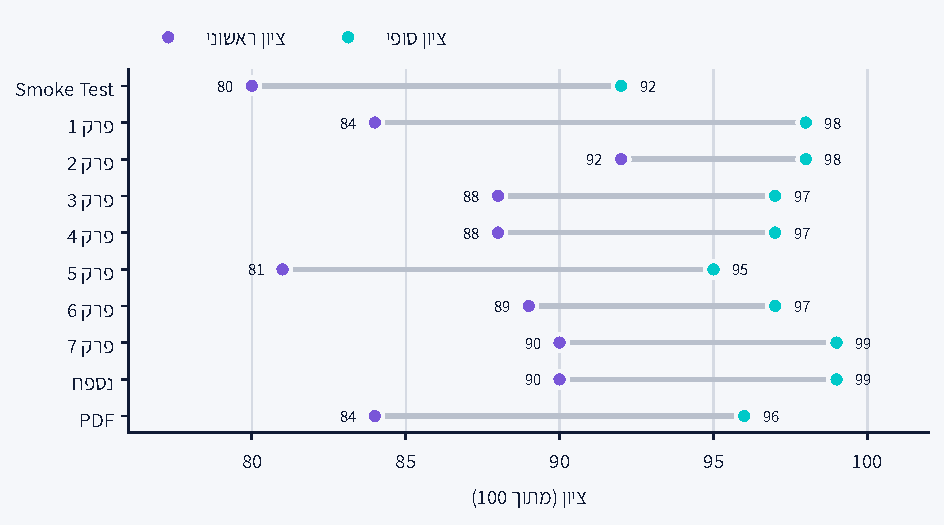
\includegraphics[width=\linewidth]{assets/charts/figA_2_scores.pdf}
\caption{ציוני הביקורת הפנימית של הסוכנים, סבב ראשון מול סבב אחרון}\label{fig:A.2}
\figurenote{מקור: python/data/review\_scores.csv}
\end{figure}
אבל ציון 96 ופסק PASS אינם סוף פסוק. אחרי שלב ההפקה העבירה המשתמשת את הספר, גרסה 0.9 בת 46 עמודים, לביקורת חיצונית ב-ChatGPT, מחוץ למערכת הסוכנים \projref{\nolinkurl{prompts/12_m5b_m6_external_review.txt}}. המבקר החדש מצא ליקויים שהלולאה הפנימית החמיצה. בעימוד: מספור עמודים, שטחים לבנים, תיבות סיכום בעמודים כמעט ריקים, חפיפות בתרשים 2.1, סימוני LaTeX גולמיים, עברית הפוכה בגרפים והביבליוגרפיה \projref{\nolinkurl{docs/INCIDENTS.md}, IR-14 עד IR-17}. ובמדע: מקור מדויק לפונקציית tanh וקביעות גורפות מדי עליה, ערבוב בין שגיאת הכללה לפער הכללה, הגדרות לא מדויקות של התאמת יתר ותת-התאמה, תיאור של קבוצת הבדיקה שלא תאם את הקוד במלואו, וההסתברויות של "כל השאר" בגרף הטמפרטורה.
גם להערות האלה לא האמינו על סמך המילה. סוכן המחקר חזר למקורות ומצא שבעניין שגיאת ההכללה הביקורת צודקת רק בחלקה: יש חוקרים שמכנים כך את הפער עצמו, אבל "פער הכללה" חד יותר, ובו בחר הספר \projref{\nolinkurl{agents/runs/research_m5b_r1.md}}. רוב ליקויי העימוד היו שיטתיים, ולכן תוקנו בכלים וקיבלו בדיקות חדשות. והלקח: מודל אחר, שלא השתתף בכתיבה, ראה מה שמערכת שבודקת את עצמה לא ראתה.
\section{האדם שמעל הלולאה}
המבנה עצמו נולד מדרישה של המשתמשת שהובילה את הפרויקט: ארבעה סוכנים ומבנה כוכב \projref{\nolinkurl{docs/PROMPT_HISTORY.md}, רשומה 002}. היא בחרה את הפלטה ואת רוח הכתיבה, והחליטה שהנספח הזה ייכתב \projref{\nolinkurl{docs/PROMPT_HISTORY.md}, רשומות 006–007}. פרק 1 נכתב לבדו, והעבודה נעצרה. רק אחרי שאישרה את הפרק ואת הסגנון נכתבו שאר הפרקים \projref{\nolinkurl{docs/PROMPT_HISTORY.md}, רשומות 007–008}.
הסוכנים אינם צוות של אנשים. הם מופעים של מערכת בינה מלאכותית, והראיה למה שעשו אינה ההצהרות שלהם אלא התיעוד. כל פרומפט וכל פלט גולמי נשמרו בתיקיית agents/runs. גם הנספח הזה נכתב בידי סוכן הכתיבה, וגם הוא עובר ביקורת.
ולבדיקה יש מחיר. עד סוף שלב ההפקה תועדו 51 הפעלות של תתי-סוכנים, ול-48 מהן נרשם מספר טוקנים: 3,511,855 בסך הכול. הביקורת לבדה צרכה 1,408,658, יותר מהכתיבה (1,277,930) \projref{\nolinkurl{agents/runs/}}. כדי לחסוך הופעל סוכן אחד בכל רגע, לבקשת המשתמשת \projref{\nolinkurl{docs/PROMPT_HISTORY.md}, רשומה 010}. משימות נמסרו בקבצים ולא בהקשר ארוך, בדיקות האיכות רצו בקוד, והמאתר והמתקן עברו פעם אחת על הספר כולו ולא על כל פרק בנפרד. הביקורת הסופית (M6) וההעלאה (M7) עוד לפנינו.
בסוף פרק 7 מה שתפח היה שיקול הדעת של הקוראת. גם הספר תפח באותה דרך, לאט ובשכבות: טיוטה בטוחה מדי, עין זרה שבודקת, תיקון, ושוב בדיקה. ההבדל היחיד הוא שכאן כל שכבה נשמרה בקובץ, כדי שגם אתם תוכלו לבדוק.
\begin{insightsbox}
\begin{itemize}
\item הפרדת תפקידים היא מנגנון בקרה: מי שכותב אינו מחפש מקורות, ומי שמבקר אינו מתקן.
\item קובץ שעובר מיד ליד משאיר עקבות; שיחה ישירה בין סוכנים לא הייתה משאירה.
\item גם מקור מכובד יכול לסתור את עצמו, ורק קריאה בנתונים עצמם חושפת זאת.
\item התקרה של סבבי התיקון אינה מגבלה טכנית, אלא החלטה איפה מכונה מפסיקה ואדם מתחיל.
\item התאוששות מתקלה מתחילה בבדיקה של מה שבאמת קיים, ולא במה שזוכרים שנעשה.
\item ציון פנימי גבוה אינו סוף הבדיקה: עין מבחוץ מצאה מה שהלולאה החמיצה, וליקוי שחוזר בכל מקום מתקנים בכלי שיצר אותו.
\end{itemize}
\end{insightsbox}


\backmatter
\chapter*{רשימת מקורות}
\addcontentsline{toc}{chapter}{רשימת מקורות}
\markboth{רשימת מקורות}{}
המקורות ממוספרים לפי סדר הופעתם הראשונה בספר, בסגנון IEEE. המספר בסוגריים מרובעים בגוף הטקסט מפנה לרשומה כאן.
\begin{english}
\printbibliography[heading=none]
\end{english}

\end{document}
